\documentclass[11pt]{article}

% general packages without options
\usepackage{amsmath,amssymb,bbm,amsfonts,amsthm}
\usepackage{commath}
% graphics
\usepackage{graphicx}
% text formatting
\usepackage[document]{ragged2e}
\usepackage{pagecolor,color}

\newcommand{\noun}[1]{\textsc{#1}}

\usepackage[utf8]{inputenc}
\usepackage[T1]{fontenc}
% geometry
\usepackage[margin=1.8cm]{geometry}

\usepackage{multicol}
\usepackage{setspace}



\usepackage{natbib}
\setlength{\bibsep}{0.0pt}

\usepackage[french]{babel}

% layout : use fancyhdr package
%\usepackage{fancyhdr}
%\pagestyle{fancy}

% variable to include comments or not in the compilation ; set to 1 to include
\def \draft {1}


% writing utilities

% comments and responses
%  -> use this comment to ask questions on what other wrote/answer questions with optional arguments (up to 4 answers)
\usepackage{xparse}
\usepackage{ifthen}
\DeclareDocumentCommand{\comment}{m o o o o}
{\ifthenelse{\draft=1}{
    \textcolor{red}{\textbf{C : }#1}
    \IfValueT{#2}{\textcolor{blue}{\textbf{A1 : }#2}}
    \IfValueT{#3}{\textcolor{ForestGreen}{\textbf{A2 : }#3}}
    \IfValueT{#4}{\textcolor{red!50!blue}{\textbf{A3 : }#4}}
    \IfValueT{#5}{\textcolor{Aquamarine}{\textbf{A4 : }#5}}
 }{}
}

% todo
\newcommand{\todo}[1]{
\ifthenelse{\draft=1}{\textcolor{red!50!blue}{\textbf{TODO : \textit{#1}}}}{}
}


\makeatletter


\makeatother


\begin{document}







\title{Space and complexities of territorial systems
\\\bigskip
\textit{Actes des Journ{\'e}es de Rochebrune 2019}
}
\author{\noun{Juste Raimbault}$^{1,2,3}$
\bigskip\\
$^1$ UPS CNRS 3611 ISC-PIF\\
$^2$ CASA, UCL\\
$^3$ UMR CNRS 8504 G{\'e}ographie-cit{\'e}s
}
\date{}


%\pagenumbering{gobble}



\maketitle

\justify

\begin{abstract}
	The spatial character of territorial systems plays a crucial role in the emergence of their complexities. This contribution aims at illustrating to what extent different types of complexities can be exhibited in models of such systems. We develop from a theoretical viewpoint some arguments illustrating ontological complexity, in the sense of the diversity and multidimensionality of possible representations, and then complexity in the sense of emergence, i.e. the necessity of the existence of several autonomous levels. We then propose numerical experiments to explore properties of complexity (dynamical complexity and co-evolution) within two simple models of urban morphogenesis. We finally suggest other dimensions of complexity which could be typical of territorial systems.\medskip\\
	\noindent\textbf{Keywords: }\textit{Complexities; Territorial systems; Urban morphogenesis; Co-evolution}
\end{abstract}





\section{Introduction}


Territorial systems, which can be understood as self-organized socio-spatial structures  \citep{pumain1997pour}, are an archetypal of complex systems studied by numerous approaches which include more or less the spatial aspect of these systems. Our interpretation of territorial systems is more particularly situated within the heritage of the evolutionary urban theory~\citep{pumain2018evolutionary} which understands urban systems as multi-level systems, in which the co-evolution of multiple components and agents determine their dynamics~\citep{raimbault2018caracterisation}. The complexity of these systems is thus closely linked to their spatial nature, since their dynamics are carried within the spatial distribution of their entities and sub-systems, and interactions between agents causing the emerging behavior are embedded in space.


The concept of complexity corresponds to various approaches and definitions, which depend on the domains in which they were introduced. For example, \cite{chu2008criteria} reviews the conceptual and operational approaches linked to the domain of artificial life and shows that there is no unified concept. \cite{deffuant2015visions} also develops different visions of complexity, ranging from a complexity close to a computational complexity to an irreducible complexity typical of social systems. A previous work by \cite{raimbault2018relating} has proposed to suggest epistemological bridges between different approaches and definitions of complexity, and more particularly the links between complexity in the sense of emergence, computational complexity and informational complexity. As highlighted by \cite{batty2018defining}, dimensions of complexity are potentially infinite and an approach which would be universally valid for all problems and systems can not exist. It is therefore crucial to combine different approaches of complexity to understand its role within territorial systems.

This contribution aims at illustrating an approach of territorial systems through urban geography, and to what extent their complexity is closely linked to their spatial nature. We propose here to illustrate the links between complexity and space according to different views of it, both through theoretical considerations but also through the exploration of simulation models of territorial systems. The rest of this paper is structured as follows: first in two sections we develop a conceptual approach to ontological complexity and emergence in territorial systems. We then describe results from the simulation of an urban morphogenesis model which exhibits properties typical of dynamical complexity. An other experiment allows then to show the link between complexity in the sense of a co-evolution and the spatial structure of the system. We finally discuss the implications of these results and possible developments.


%%%%%%%%%%%%%%%%%
\section{Ontological complexity}
%%%%%%%%%%%%%%%%%


A first theoretical approach allows to tackle what we call \emph{ontological complexity}, which was proposed by \cite{pumain2003approche} as the broadness of disciplinary viewpoints necessary to apprehend a common object. The multidimensionality of territorial systems remains a main issue for their understanding, as show \cite{perez2016agent} in the case of multi-agent systems. Thus, interdisciplinarity would be intrinsic to ``urban sciences'', i.e. to the different disciplines considering the city as an object of study, although it is in practice difficult and subject to the contingency of the social organisation of sciences \citep{dupuy2015sciences}.


We take the example of \cite{raimbault2017invisible} as a proof-of-concept of the diversity of approaches possible in the case of interactions between networks and territories, and suggest hypotheses regarding the role of space in this complexity, such as the evolutive processes of diversification and specialization linked to spatial niches. More precisely, \cite{raimbault2017invisible} establishes a scientific map of modeling approaches to interaction between transportation networks and territories. Through a citation network analysis, complementary approaches are exhibited, including for example quantitative geography, political geography, urban economics, planning, physics. Each approach provides a particular dimension of the same system. Space leading to the differentiation of sub-systems, it seems on the one hand natural that some have a higher importance than others in the different instances, and on the other hand that complementary questionings coexist (these being in fact endogenous to territorial systems, since innovation and thus research and science are an important driver of urban systems dynamics \citep{pumain2010theorie}).


At this point we propose an hypothesis, which empirical exploration would require deeper scientometric analysis out of the scope of this work, according to which a more elaborated spatialization would be linked to a broader ontological spectrum. The example of \emph{New Economic Geography} and geographical economics illustrates that aspect \citep{marchionni2004geographical}: the first approach, in order to deploy its analytical tools, imposes a strong reductionism on space (line or circle for a large part of models) and on objects (representative agents, homogeneity), whereas the second will favor empirical descriptions more faithful to geographical particularities. It is difficult to know if space is richer because the approach is not reductionist or the contrary, that a rich space increases ontological range. Pretend a sense of causality would in fact be counter-productive, and this congruence confirms our argument that an elaborated spatialization of models of territorial systems is correlated to a higher ontological richness.


This reflexion can be shifted to the methodological domain, within which we can highlight the tension between model precision and robustness of results, in particular by comparing agent-based models and dynamical systems models allowing a certain level of analytical tractability. The archetype of approaches in economic geography, considering an unidimensional system \citep{krugman1992dynamic}, looses the essence of space which is heterogeneity and multiplicity of alternatives, whereas precisely spatialized models such as Luti models, will necessitate simulations and a restricted validation of results \citep{bonnel2014survey}. The degree of precision of models is however not directly linked to their spatial character, as shows the comparison between agent-based models and demographic microsimulations \citep{birkin2011spatial}. However, approaches including an elaborated description of space, with the inclusion of scales for example, are mainly associated to an ontological richness in the study of these systems, which need to be maintained to ensure the diversity of knowledges on the subject \citep{sanders2018survival}.


%%%%%%%%%%%%%%%%
\section{Complexity and emergence}
%%%%%%%%%%%%%%%%


Our second theoretical entry focuses on complexity as the weak emergence of structures and autonomy of upper levels~\citep{bedau2002downward}. Weak emergence consists in the interpretation that the levels of a systems are effectively \emph{computed} \citep{morin1980methode} by itself, and that it is necessary to simulate the system to reproduce them. The diachronic aspect of dynamics allows this view of emergence to not being incompatible with downward causation. We recall the intrinsic multi-scalar aspect of territorial systems, which is highlighted for example in the approach of cities as systems within systems of cities, as introduced by \cite{pumain1997pour} which extends \cite{berry1964cities}. Furthermore, there is currently a necessity to produce spatial models integrating effectively this multi-scalar aspect~\citep{rozenblat2018conclusion}, with the aim of effectively operational models.


The difficulty to endogenize autonomous upper levels can for example be illustrated by~\cite{lenechet:halshs-01272236} which introduces a co-evolution model between transportation and land-use at the metropolitan scale integrating an endogenous governance structure for the transportation network. Simulating tractations between local actors of transportation, some regimes lead to the emergence of an intermediary governance level produced by the collaboration between neighbor actors. The three decision levels are then indeed ontologically autonomous but also in terms of their dynamics. The emergence of collaboration is finely linked to the spatial structure, since actors include accessibility patterns in their decision-making process. Less rich models of co-evolution between transport and land-use, as \cite{raimbault2018urban} at the mesoscopic scale taking into account urban form and topology of the road network, or \cite{raimbault2018modeling} which abstract networks as distance matrices at the macroscopic scale and postulates dynamics on these, indeed capture an emergence fundamentally linked to space, but remain restricted in the articulation of levels, whereas the governance model is closer to the qualitative emergence of upper levels.


Systems with a lower ontological complexity also exhibit a crucial role of weak emergence. The local state of a traffic flow is partly a consequence of the global state of the system, in particular when important congestion patterns can be observed at the macroscopic scale. In that case, spatio-temporal patterns are again central to the emergence process \citep{treiber2010three}. In these different examples, space again play a crucial role for the presence of complexity, since auto-organization implies a spatial distribution of agents, and the levels of emergence are directly linked to spatial scales whatever the interpretation of these \citep{manson2008does}. An approach of auto-organization through morphogenesis, that will be detailed within models in the following, furthermore insists on the spatial aspect in emergence, since it links form and function \citep{doursat2012morphogenetic}, the first being necessarily spatialized.





%%%%%%%%%%%%%%%%%
\section{Dynamical complexity}
%%%%%%%%%%%%%%%%%


In this section and the following, we propose to use simulation models of urban morphogenesis to show in a concrete manner other complexities of territorial systems. The models, detailed in the following, are implemented in Netlogo \citep{wilensky1999netlogo} and in scala, and explored using the model exploration software OpenMOLE \citep{reuillon2013openmole}. All code and results is openly available on the git repository of the project at \texttt{https://github.com/JusteRaimbault/SpatialComplexity}. Simulation results are available at \texttt{https://doi.org/10.7910/DVN/LENFVH}.


The understanding of complex systems as dynamical systems with more or less chaotic attractors has been largely developed in geography \citep{dauphine1995chaos}. For example, \cite{e18060197} considers that the semantic information of an urban environment is linked to the attractors of dynamical systems ruling the dynamics of its agents. This type of approach can moreover be linked to fractal approaches of urban systems, initially introduced by \cite{batty1994fractal}, and for example more recently applied to real urban planning problems \citep{yamu2015spatial}. These questions are more generally linked to transversal questions on spatio-temporal chaos \citep{crutchfield1987phenomenology}. The understanding of the link between time and space, and the corresponding non-uniform, non-stationary, non-ergodic dynamics, remains in construction on the theoretical, methodological and empirical dimensions, and promises numerous applications for the study of territorial systems. For example, \cite{chen2009urban} combines cross-correlations and Fourier analysis to study an urban gravity model. An important research direction in that frame is the understanding of the non-stationarity of territorial systems properties, and \cite{raimbault2018urban} explores it in the case of urban morphology and network topology.

% TODO : ajouter edge of chaos ?


We use here an urban morphogenesis model introduced by \cite{raimbault2018calibration} to illustrate the properties of sensitivity to initial conditions and path-dependancy of territorial systems~\citep{pumain2012urban}. In particular, we show the strong sensitivity of final simulated urban forms to spatial perturbations, and more generally the path-dependancy of trajectories for aggregated morphological indicators. This relatively simple model simulates population growth on a grid, through the iterative addition of population, which localizes following a preferential attachment to the already distributed population and diffuses in space. Important parameters are $N_G$ the exogenous growth rate, $P_{max}$ the total final population, $\alpha$ the preferential attachment exponent, $\beta$ the diffusion rate and $n_d$ a number of diffusions for each time step.


The experiment done by \cite{raimbault2018calibration} on a simplified one-dimensional version of the model shows that semi-stationary distributions of populations can be at a maximal distance (in a sense of a L2 norm between distributions) starting from a same initial configuration. In two dimensions, the phenomenon is identical as shown by the experiment done here. The model is simulated starting from an initial configuration which is particularly sensitive, constituted by four initial centers of similar size. For a grid of size 100, four centers are positioned in the middle of each cadrant, with an exponential kernel for population of the form $P_0 \cdot \exp \left(-r/r_0\right)$ with $P_0 = 100$ and $r_0 = 5$. The model is then simulated for given values of parameters for aggregation $\alpha$, diffusion $\beta, n_d$, growth and population $N_G, P_{max}$ (voir \cite{raimbault2018calibration}), and a realization of the distance between configurations $d(t)$ is computed on two independent realizations of populations $P^{(k)}_i(t)$, as $d(t)=\norm{P^{(1)}_i(t) - P^{(2)}_i(t)}$. A direct experience plan is achieved, with a LHS sampling of 390 parameter points and 1000 repetitions.


%      adjr2           lambda1           lambda2               ids             id           alpha       
% Min.   :0.5332   Min.   :0.05242   Min.   :0.0009514   Min.   :2382   Min.   :2382   Min.   :0.5016  
% 1st Qu.:0.9261   1st Qu.:0.14034   1st Qu.:0.0091442   1st Qu.:2974   1st Qu.:2974   1st Qu.:0.9059  
% Median :0.9555   Median :0.25679   Median :0.0148210   Median :3458   Median :3458   Median :1.4044  
% Mean   :0.9372   Mean   :0.31340   Mean   :0.0220534   Mean   :3454   Mean   :3454   Mean   :1.4210  
% 3rd Qu.:0.9722   3rd Qu.:0.44971   3rd Qu.:0.0275092   3rd Qu.:3963   3rd Qu.:3963   3rd Qu.:1.9154  
% Max.   :0.9888   Max.   :0.84750   Max.   :0.2040800   Max.   :4407   Max.   :4407   Max.   :2.4924  
 %     beta                 nd        relgrowthrate        growthrate      population   
% Min.   :0.0001532   Min.   :1.003   Min.   :0.005373   Min.   :500.5   Min.   :10285  
% 1st Qu.:0.1129967   1st Qu.:1.947   1st Qu.:0.010791   1st Qu.:631.5   1st Qu.:30425  
% Median :0.2408924   Median :2.884   Median :0.014974   Median :764.0   Median :50103  
% Mean   :0.2420500   Mean   :2.952   Mean   :0.019731   Mean   :761.0   Mean   :51729  
% 3rd Qu.:0.3665757   3rd Qu.:3.959   3rd Qu.:0.024075   3rd Qu.:886.5   3rd Qu.:70556  
% Max.   :0.4999998   Max.   :4.999   Max.   :0.086181   Max.   :999.7   Max.   :99790
%summary(breaks)
%   Min. 1st Qu.  Median    Mean 3rd Qu.    Max. 
%  2.492   6.947   9.389  10.701  12.732  37.020 

We show in Fig.~\ref{fig:lyapounov} a basic estimation of Lyapounov exponents, achieved with piecewise linear regression estimation on two segments, of $\log d(t)$ as a function of $t$, on all repetitions for one parameter point. The adjustment is relatively good since the first quartile of the adjusted $R^2$ is at 0.92 and its average at 0.93. The Lyapounov exponent on the first segment, that we write $\lambda_1$, varies between 0.05 and 0.84 with an average of 0.31. Thus, the quality of the adjustment and the positive values show the strong sensitivity to initial conditions of generated configurations. Temporal regimes are quite different, since the estimated breakpoint time $t_b$ varies between 2.5 and 37.0. Values of $\lambda_2$ are lower, with an average at 0.02. There exists a first regime during which the most of the urban structure is constituted followed by a second regime (that we can describe as ``semi-stationary'') during which evolutions are smaller. This moreover suggests an endogenous stopping criteria for the model. The curves of $\log d(t)$ shown in Fig.~\ref{fig:lyapounov} are for a maximal value of the adjustment and a maximal value of $\lambda_1$. We also show the variations of exponents as a function of parameters. $\lambda_1$ as a function of the aggregation $\alpha$ exhibits an unexpected behavior, relatively stable below 1.5 and then a linear increase above, without modification around 1, what suggests a threshold over which this process dramatically influences urban form. For the lower values of $\beta$, a local maximum at 1 suggests a role of the infra or supra-linear aspect of the regime. For the behavior of $\lambda_2$, a significant effect is observed only for the larger growth rates, and corresponds to a maximum around 1.5, i.e. that the switch to the second regime for $\lambda_1$ corresponds in this case to a better stabilization for the second phase. This study shows thus the sensitivity of urban configurations to infinitesimal perturbations (what is equivalent to a perturbation of the initial state).


%%%%%%%%%%%%%
\begin{figure}
	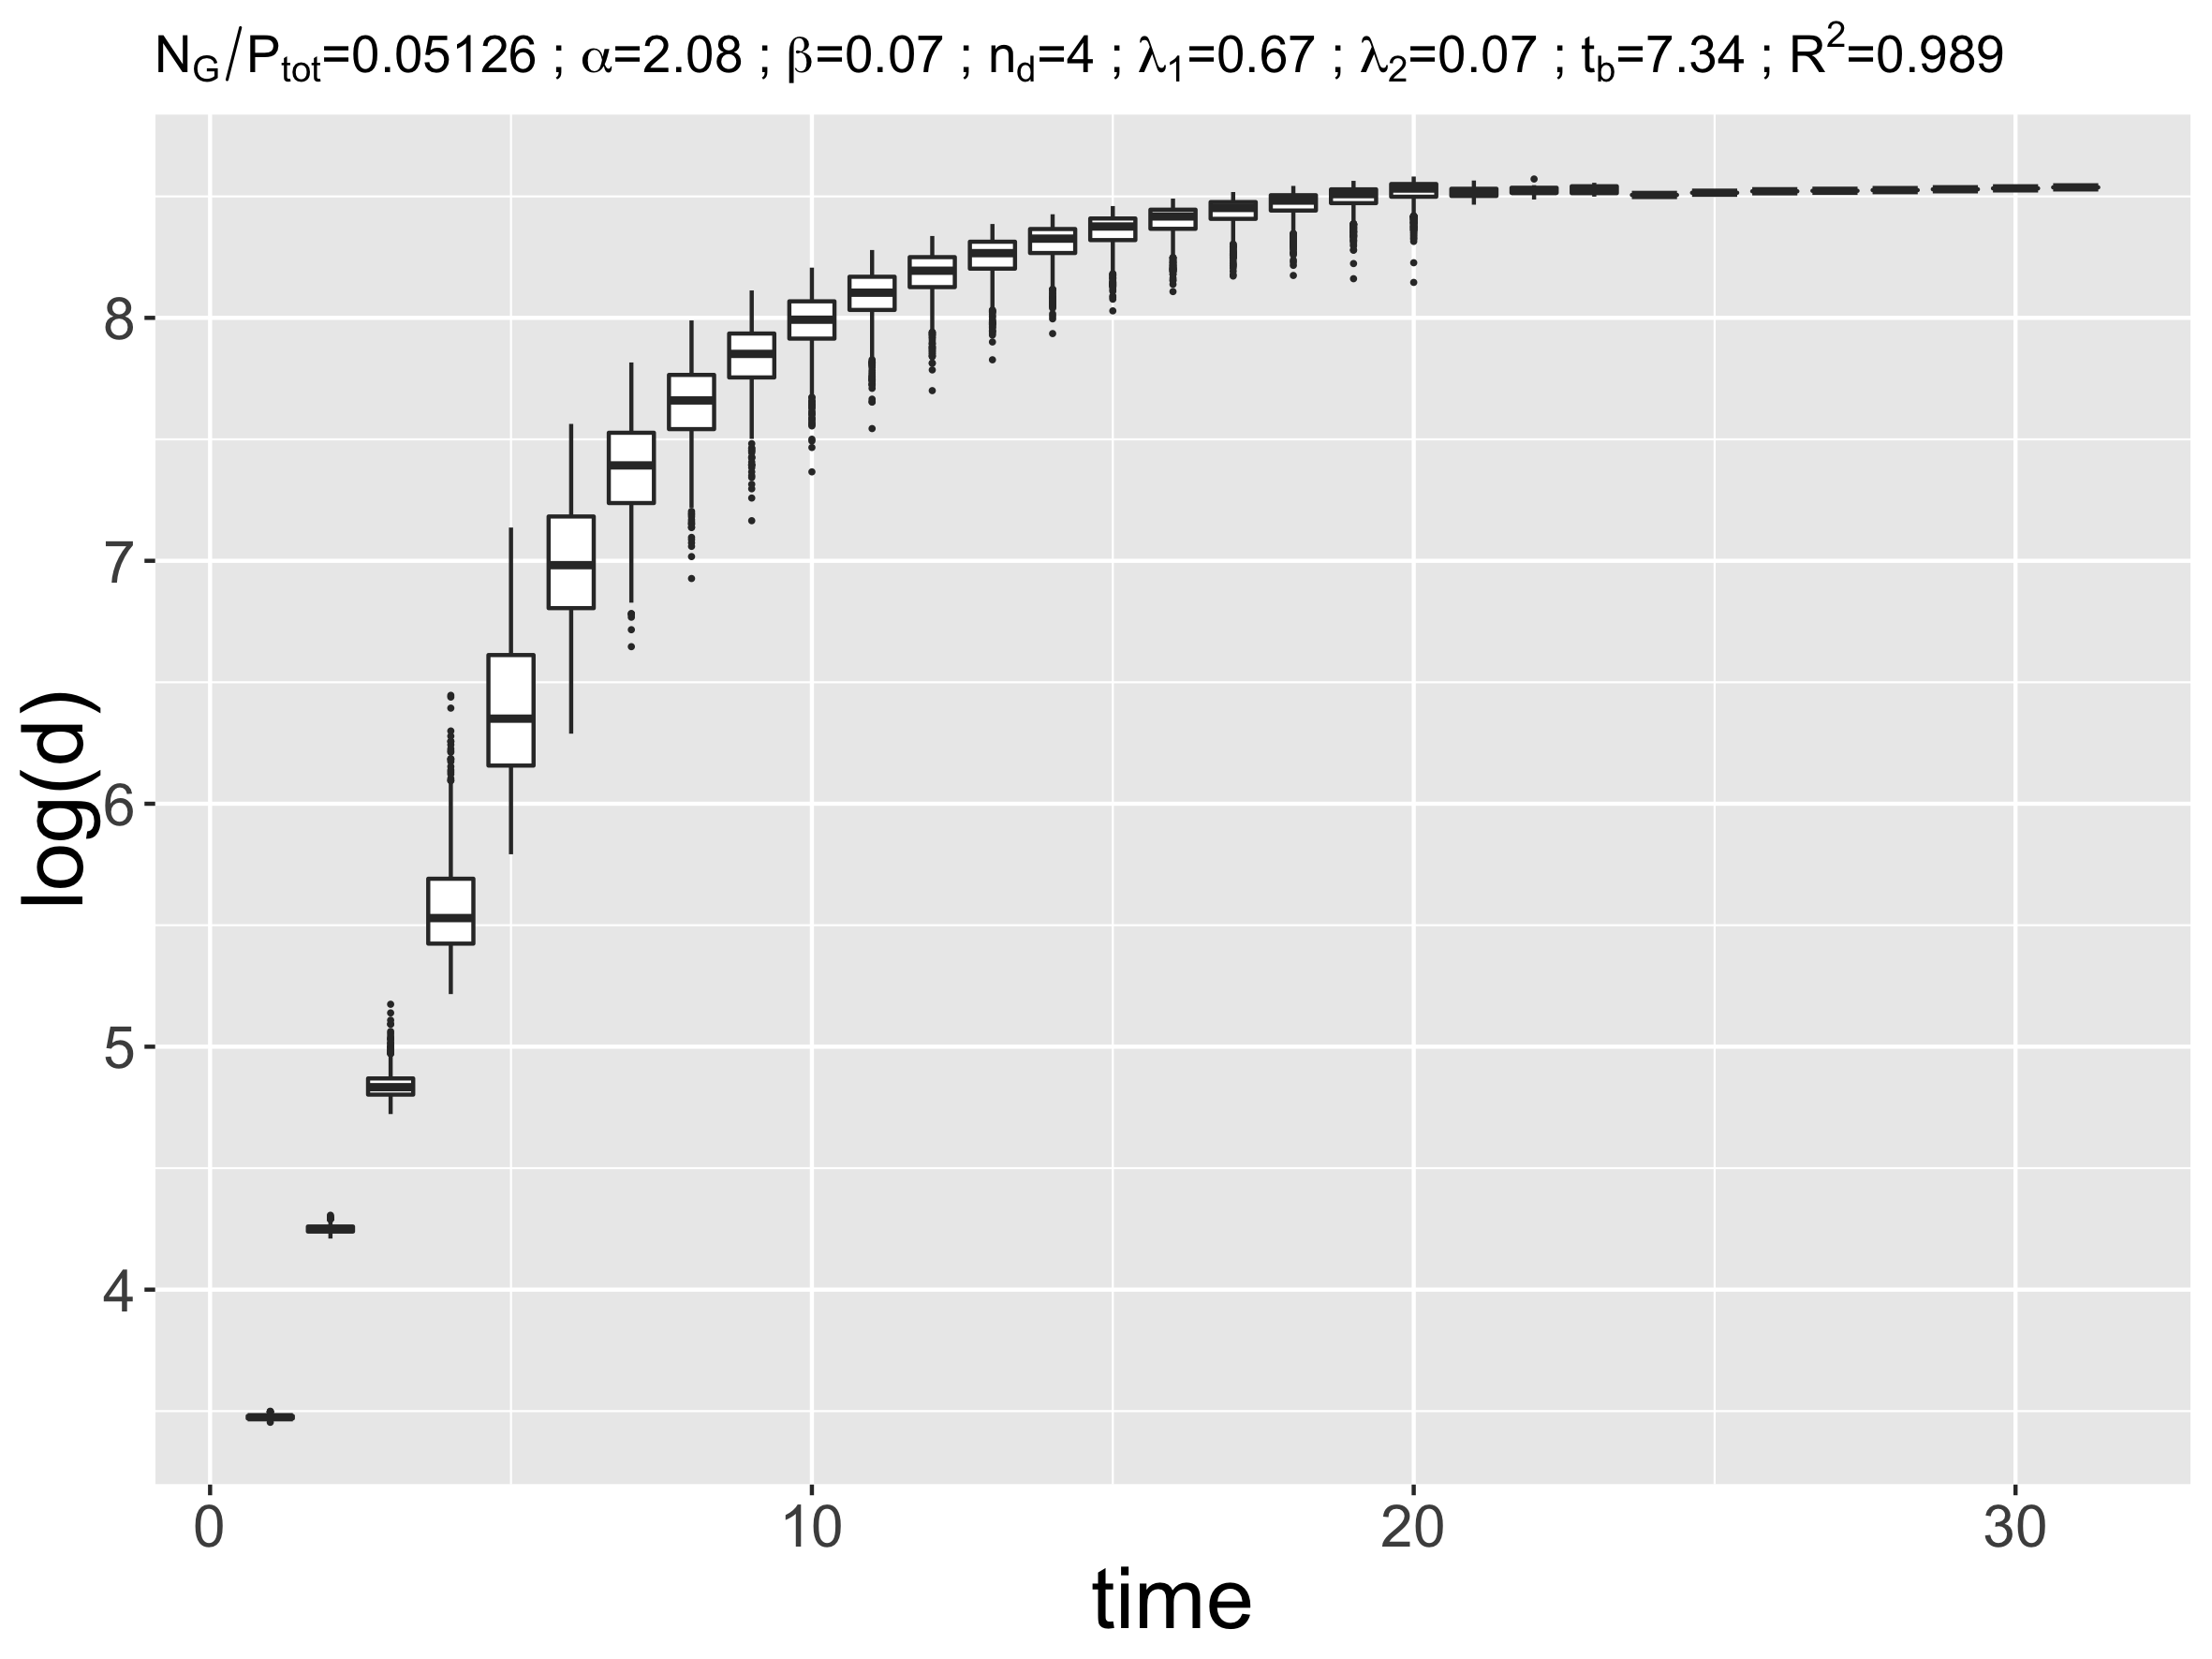
\includegraphics[width=0.49\linewidth]{figures/configdist_boxplot_id3642.png}
	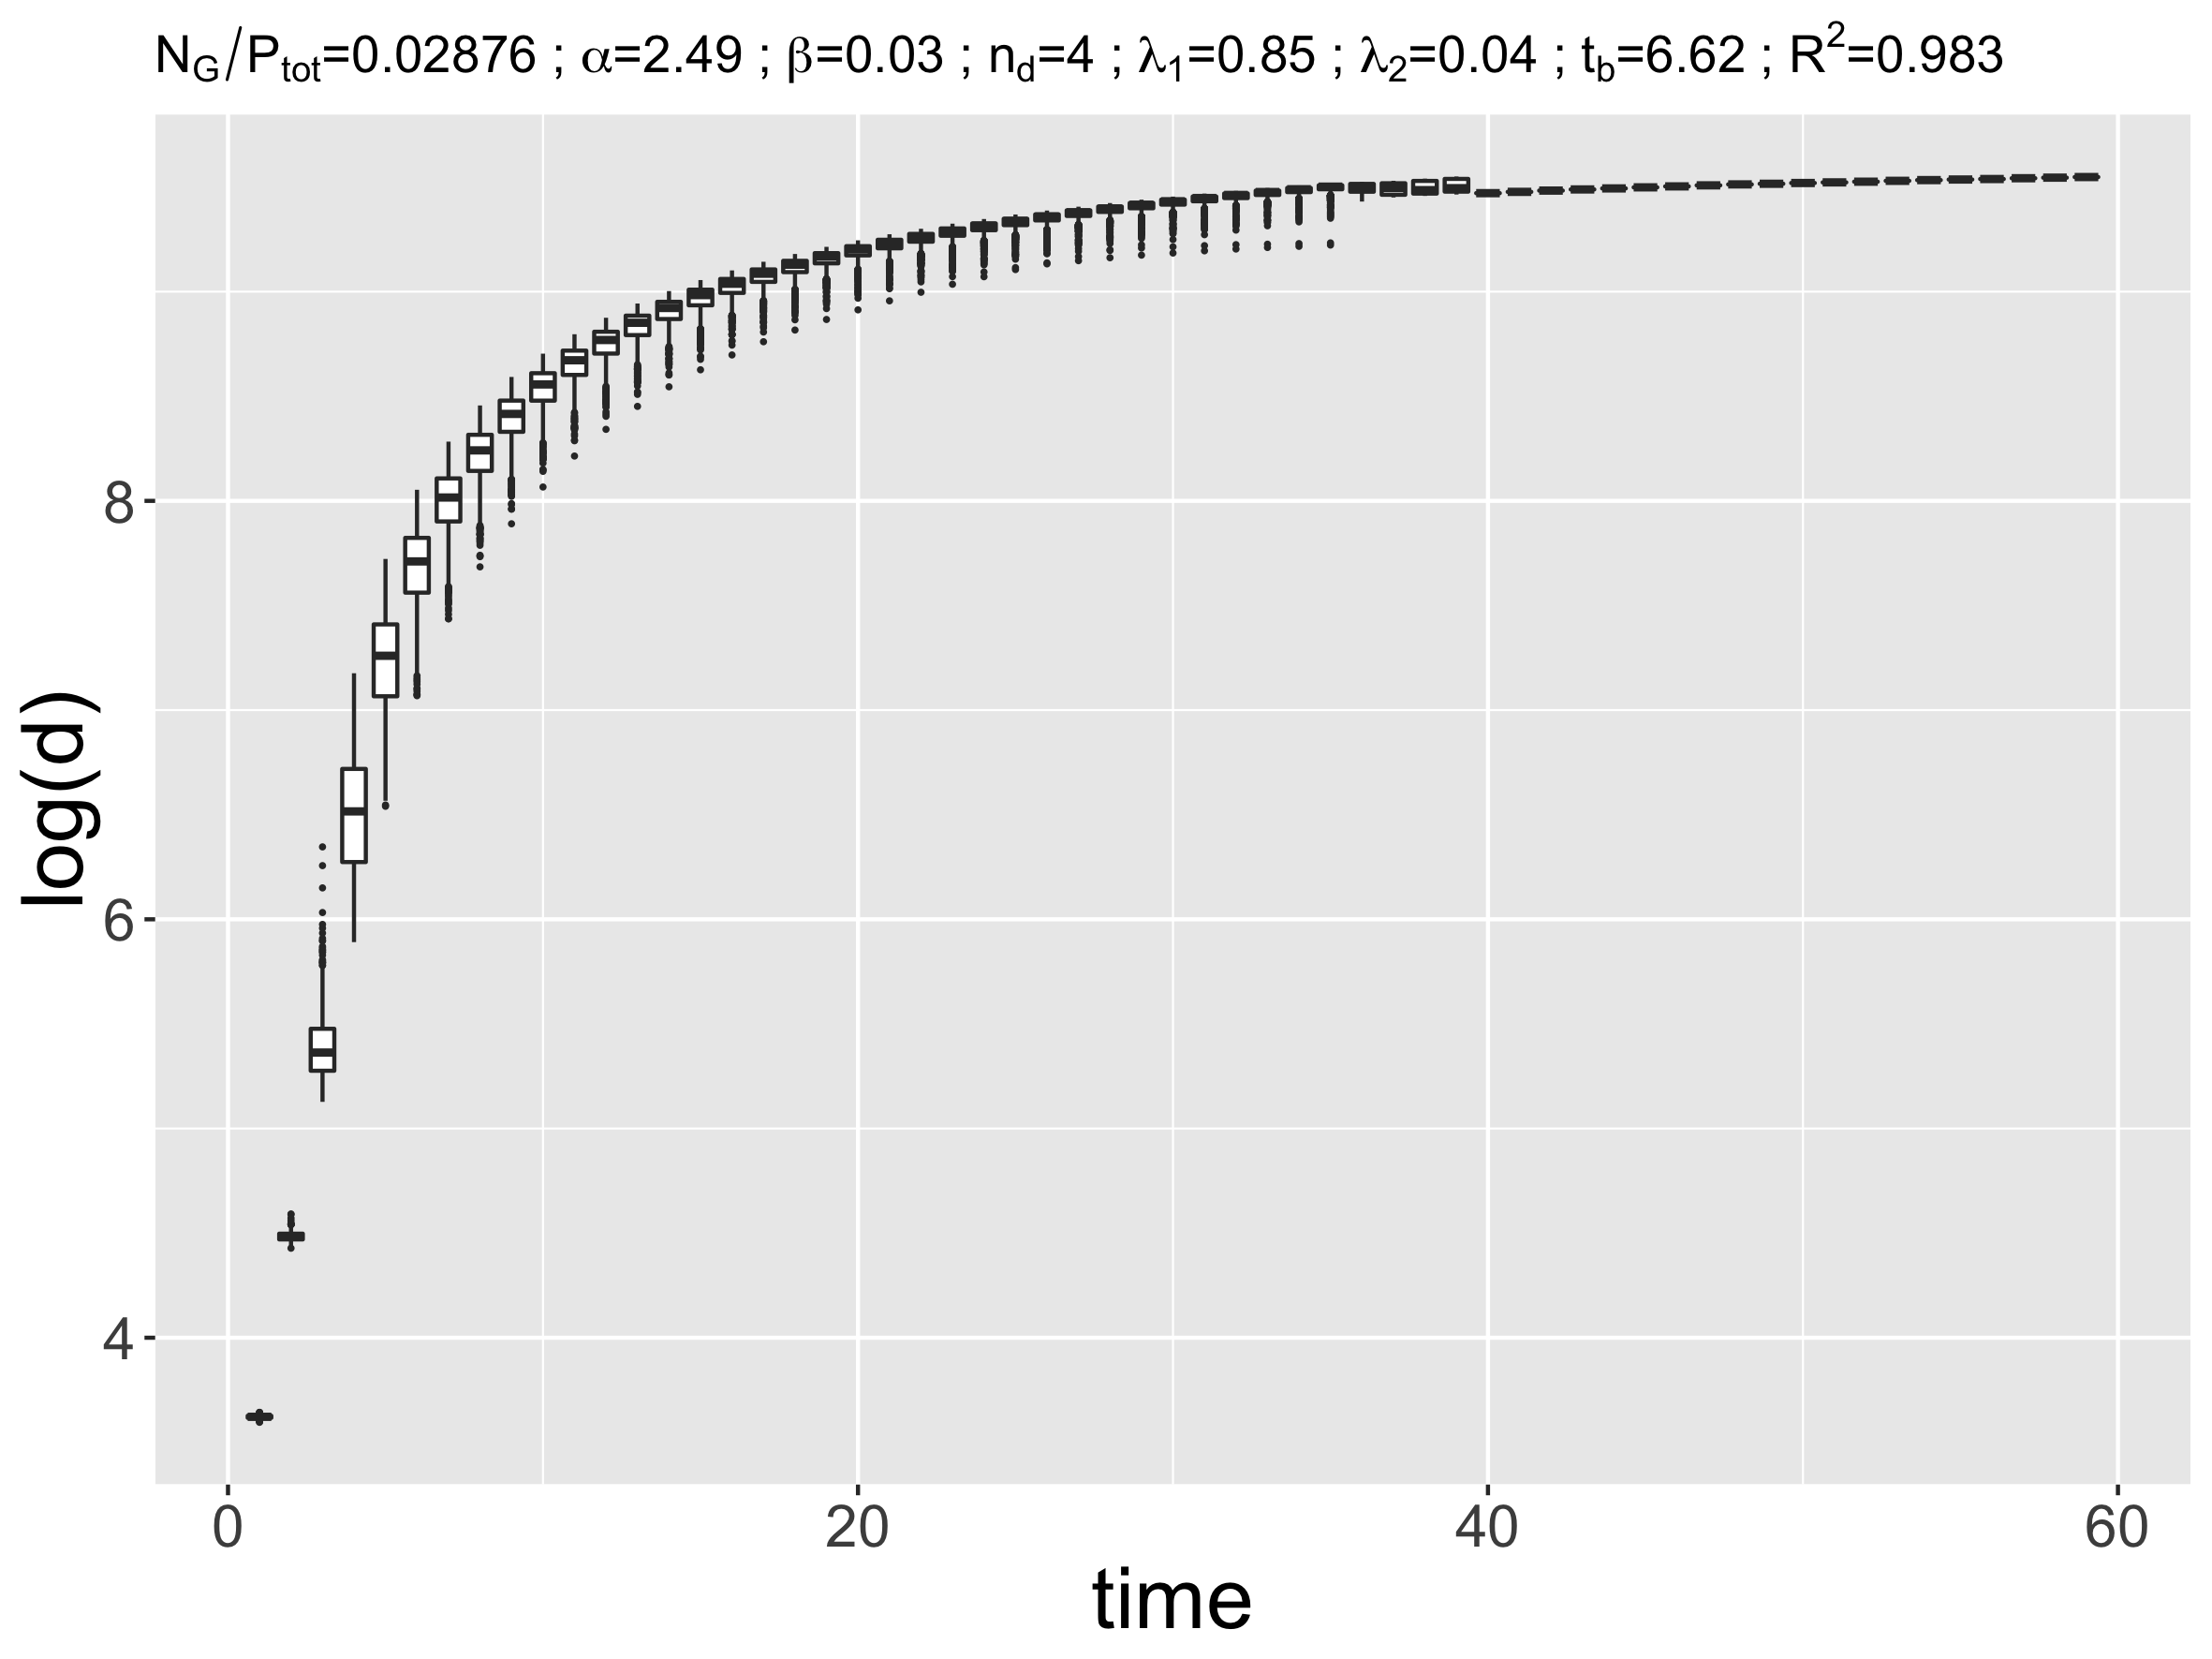
\includegraphics[width=0.49\linewidth]{figures/configdist_boxplot_id3784.png}
	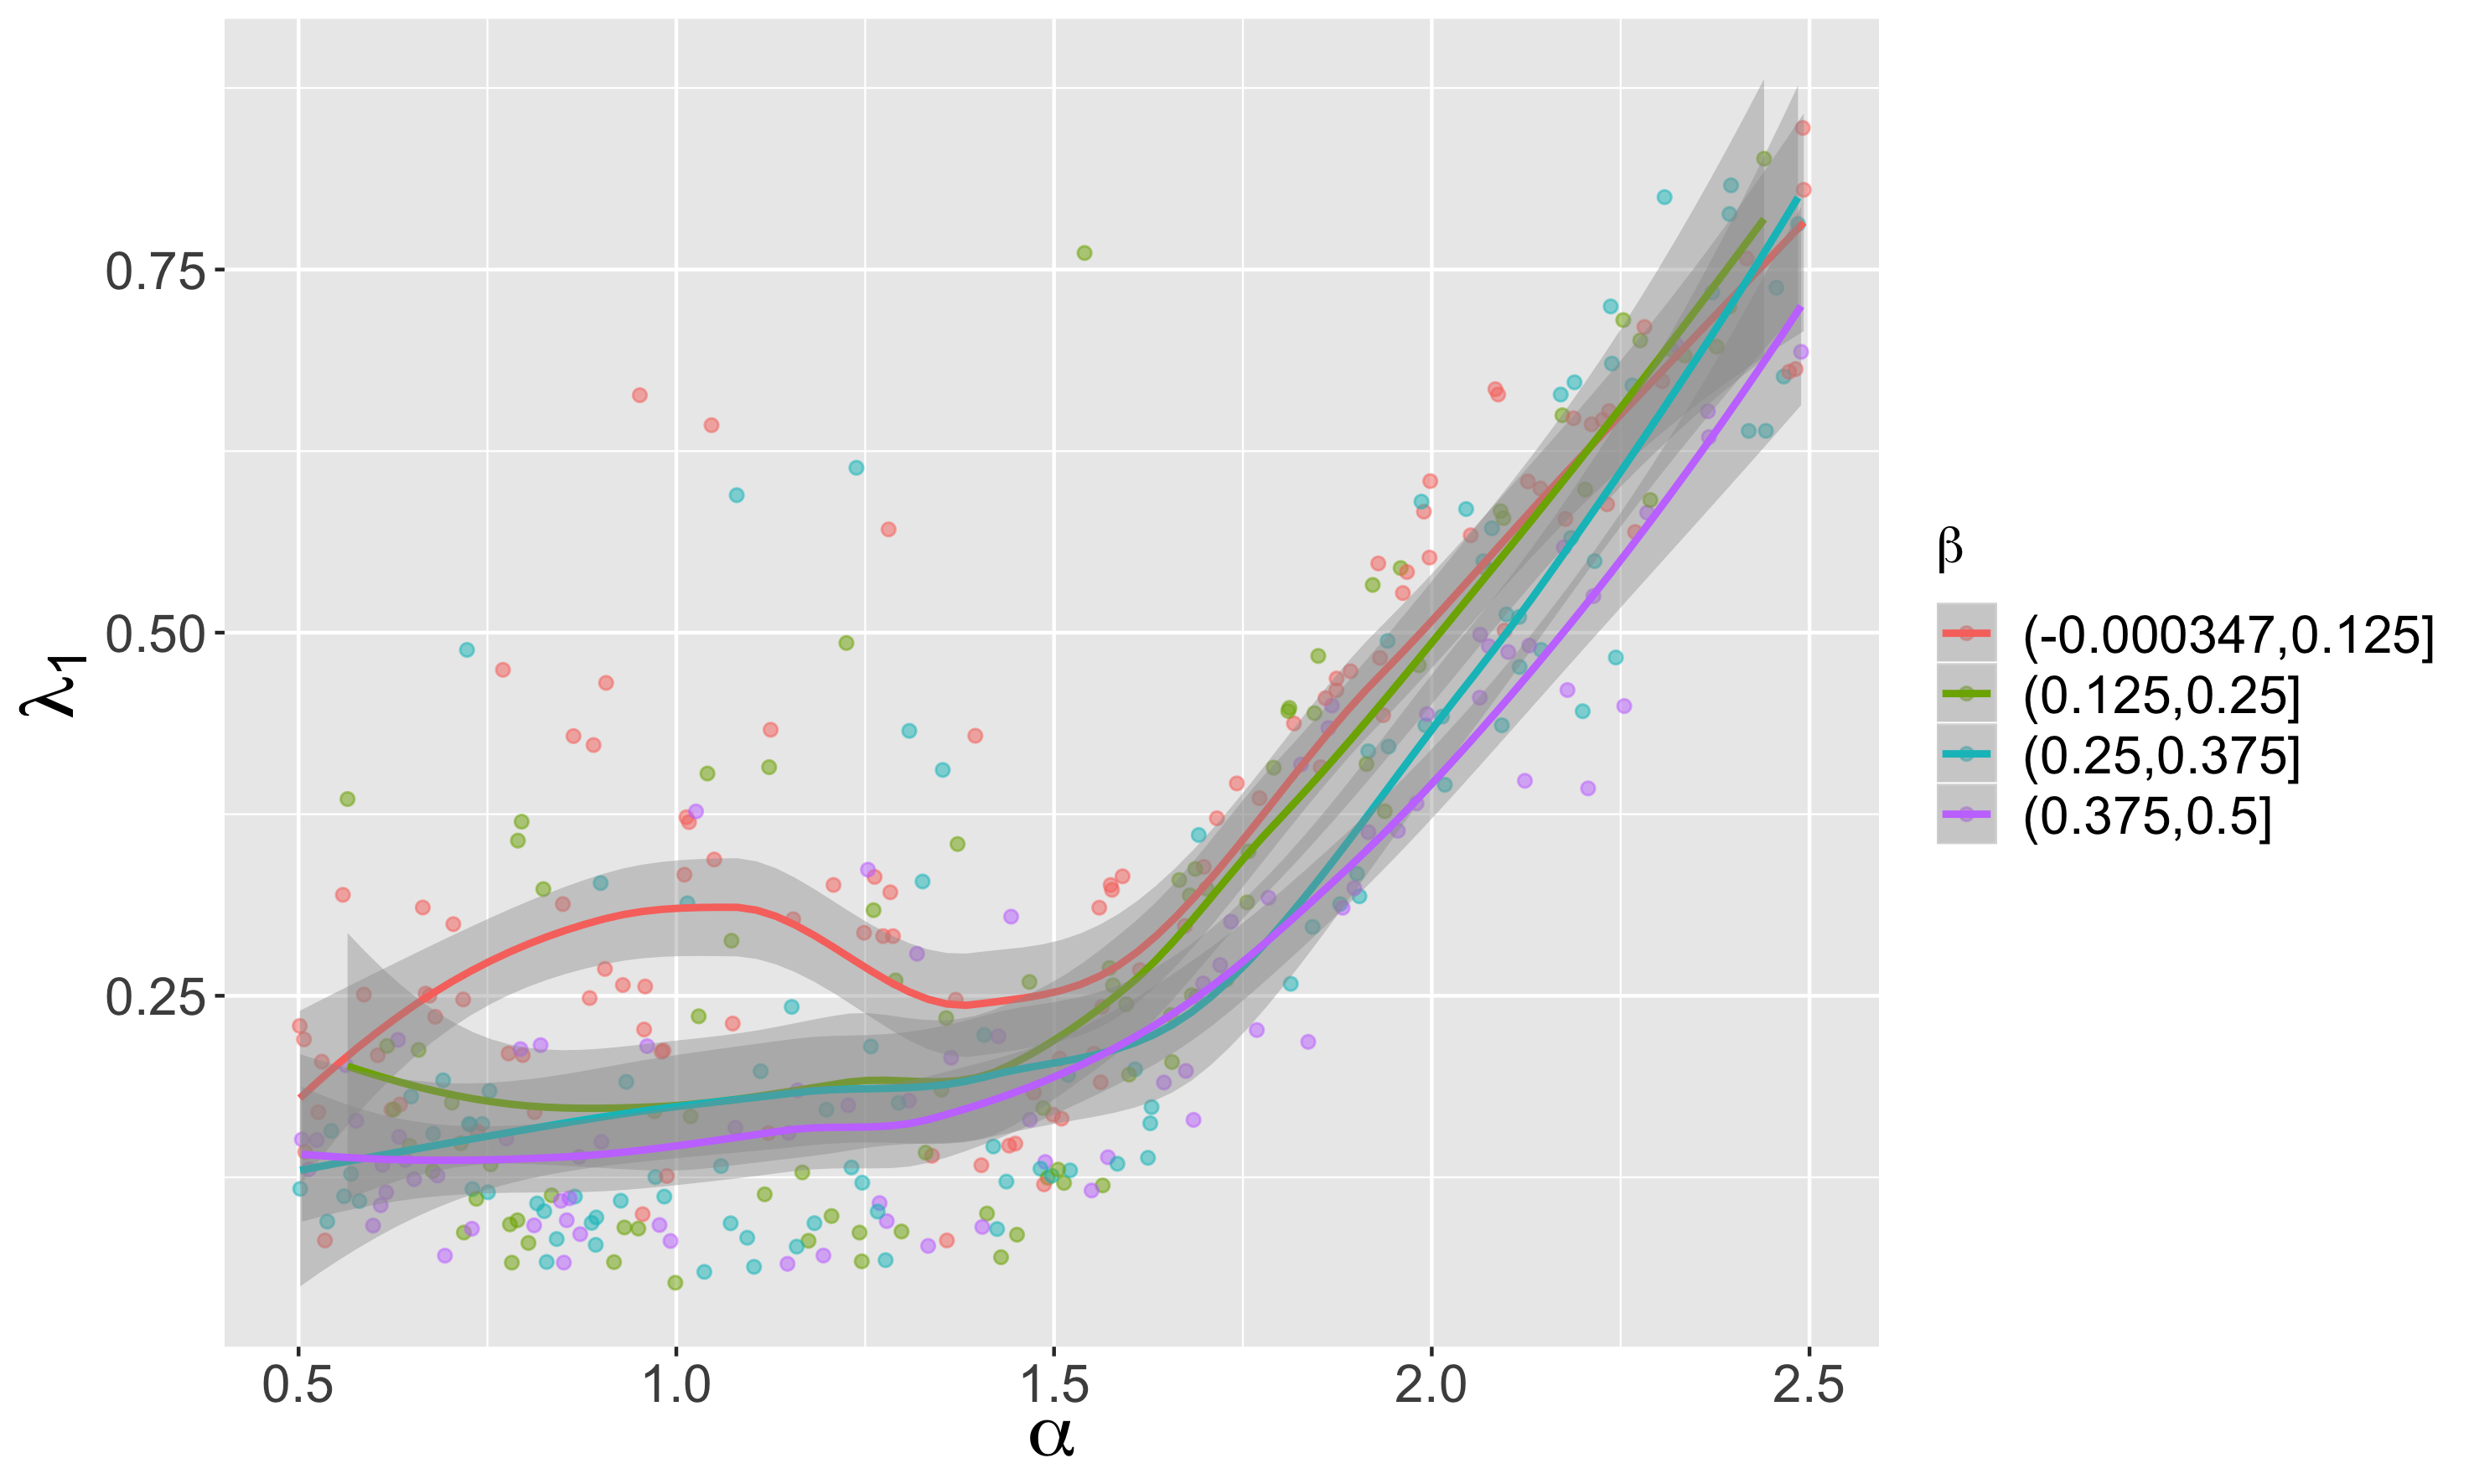
\includegraphics[width=0.49\linewidth]{figures/lambda1_alpha_colbeta.png}
	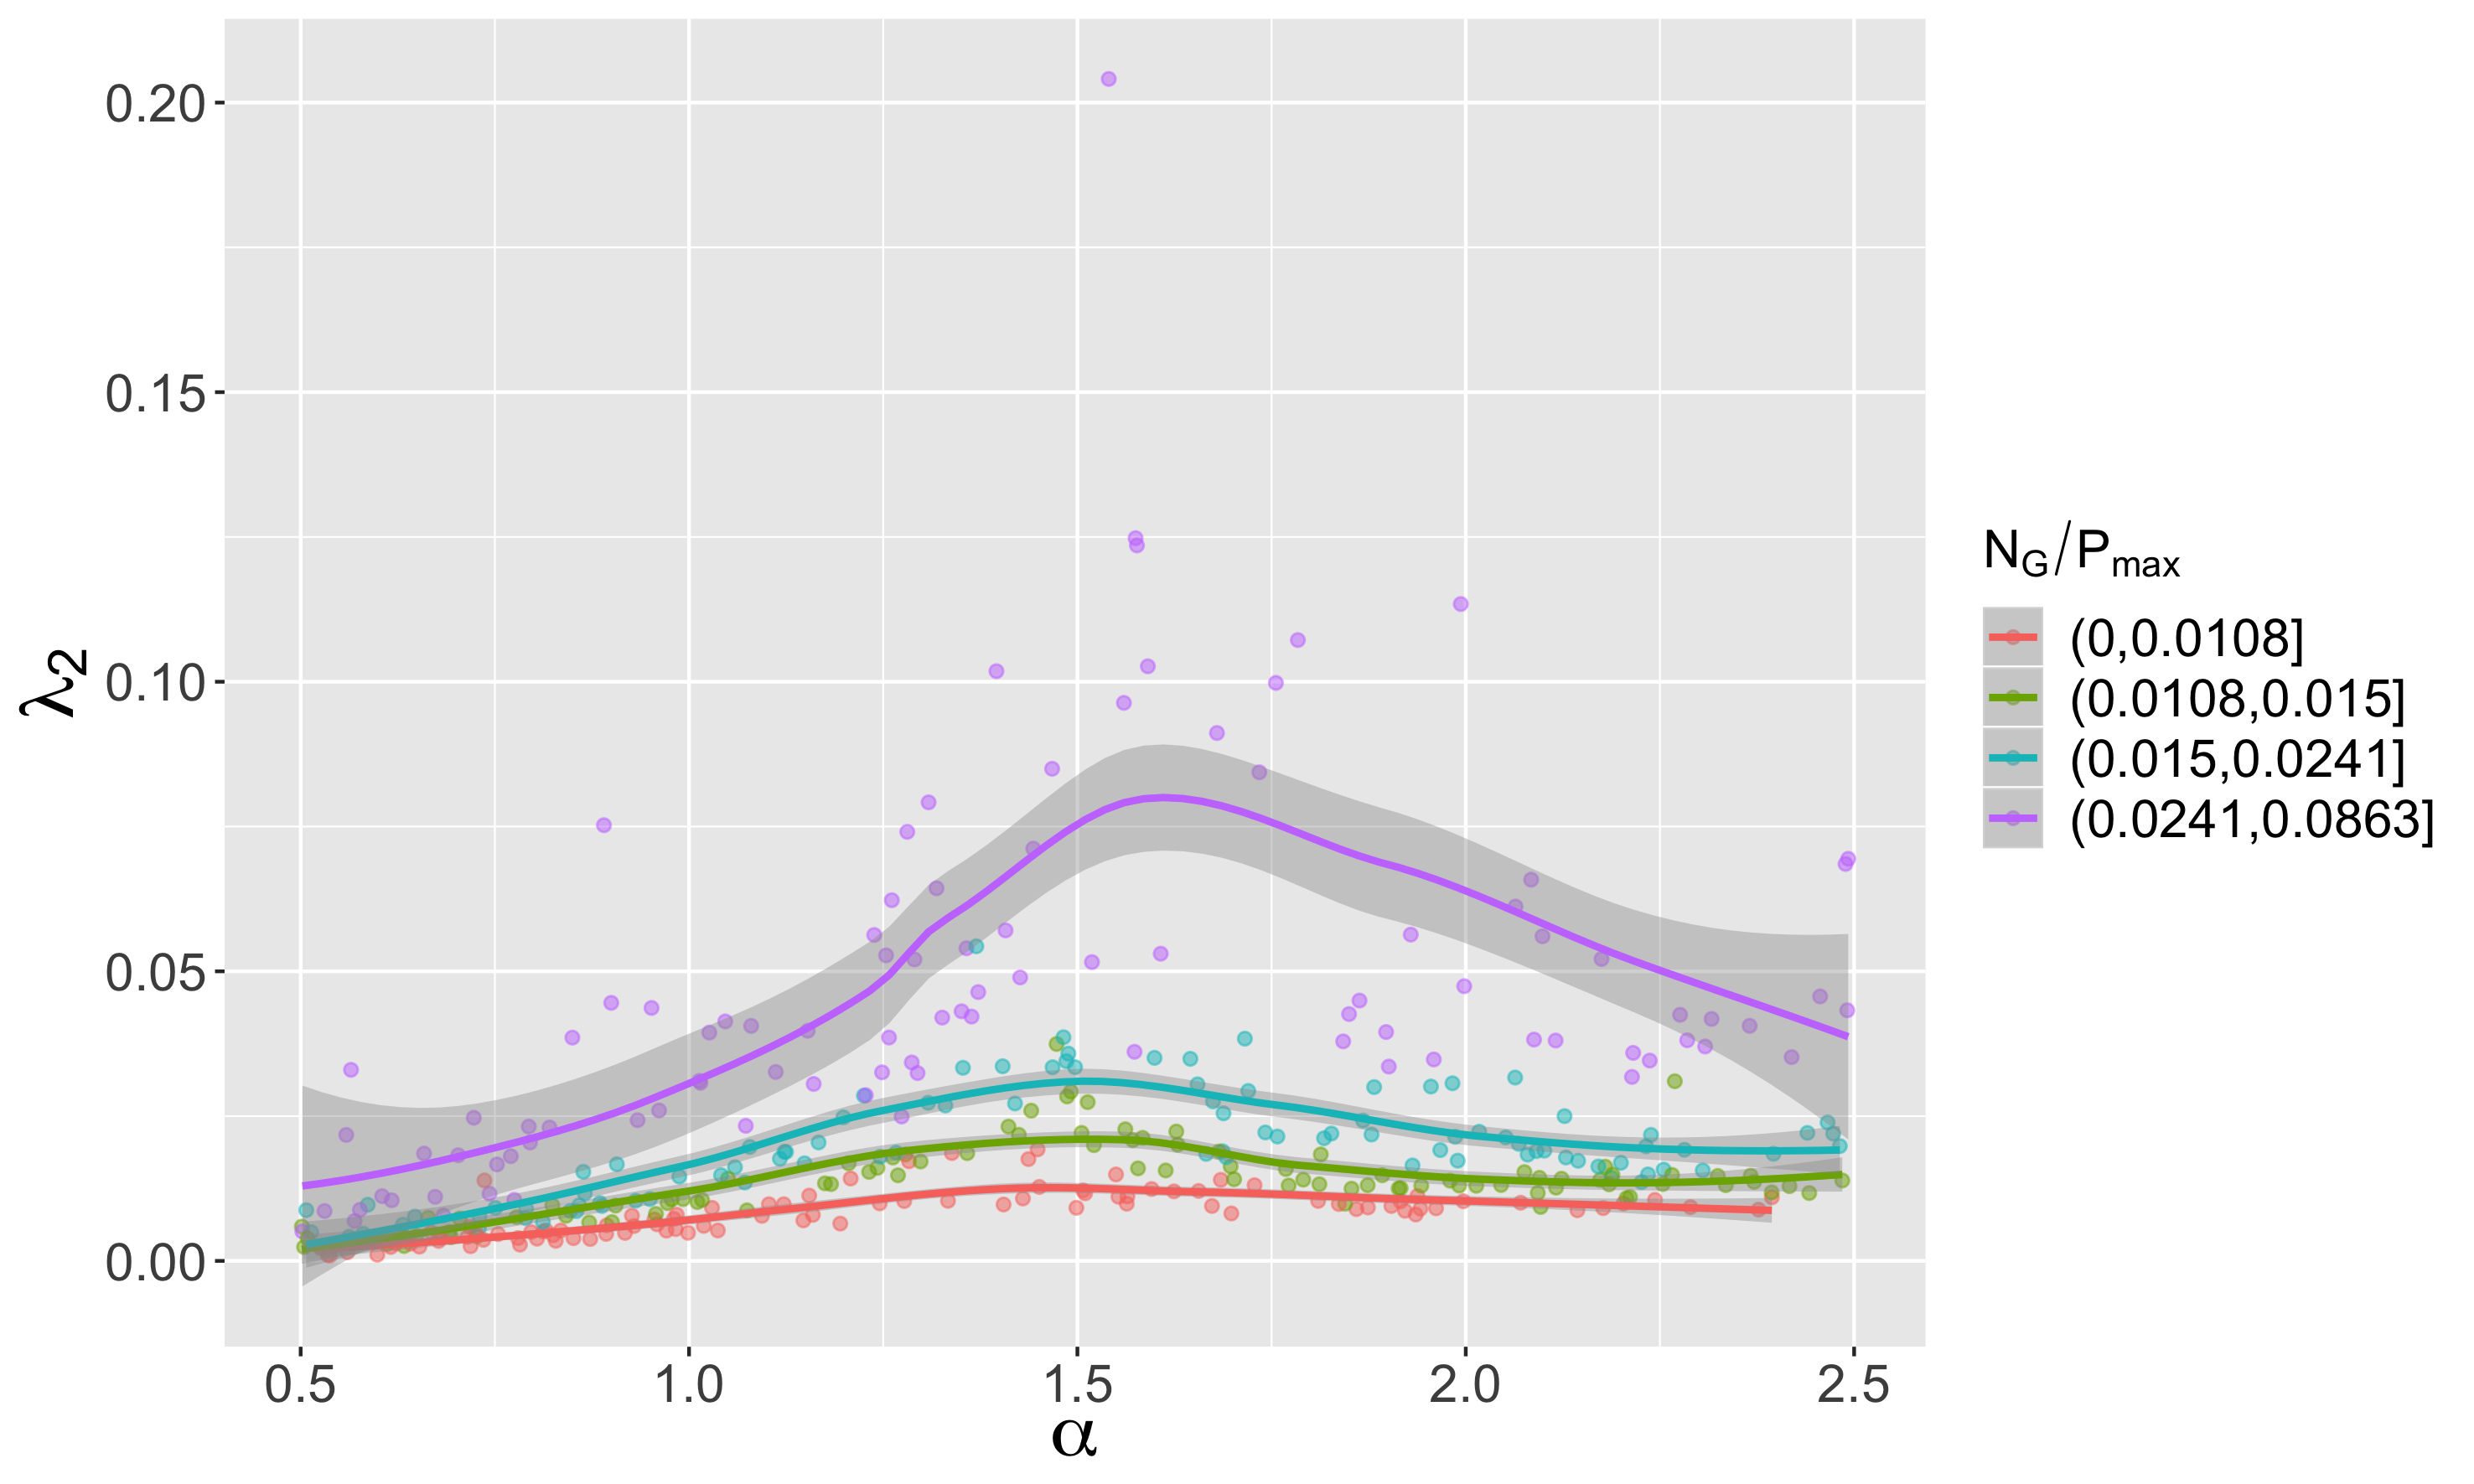
\includegraphics[width=0.49\linewidth]{figures/lambda2_alpha_colrelgrowthrate.png}
	\caption{\textbf{Estimation of local Lyapounov exponents for the reaction-diffusion model.} \textit{(Top)} Temporal profiles as descriptive statistics for $\log d(t)$ as a function of $t$, for two configurations showing a maximal fit and a maximal $\lambda_1$ value ; \textit{(Bottom left)} Value of $\lambda_1$ as a function of $\alpha$, for different values of $\beta$ (color) ; \textit{(Bottom right)} Value of $\lambda_2$ as a function of $\alpha$, for different values of $N_G / P_{max}$.}
	\label{fig:lyapounov}
\end{figure}
%%%%%%%%%%%%%


Furthermore, we illustrate the temporal trajectories of aggregated morphological indicators. A similar experience plan with a single model simulation at each repetition and an empty initial state, but following in time the values of urban form indicators (Moran, entropy, average distance, hierarchy), shows that their trajectories are path-dependent. Indeed, the example of Fig.~\ref{fig:morphotraj} shows a significant divergence of trajectories starting from the same initial point, but more importantly some trajectories crossing (indicators may therefore not be formulated as a deterministic dynamical system in which trajectories may not cross because of the Cauchy-Lipschitz theorem), exhibiting numerous points where urban form is very close (at least for the two indicators shown) for two trajectories, but the past and the future are different. Therefore, the future state of an urban system entirely depends on the past trajectory, and two systems which are very similar at a given time may exhibit fundamentally different trajectories. It is naturally an illustration with a toy model, on the particular aspect of urban form, but the path-dependence effects are a priori even more important when taking into account the multiple levels, political aspects, and infrastructures \citep{pumain2012urban}.


%%%%%%%%%%%%%
\begin{figure}
	\centering
	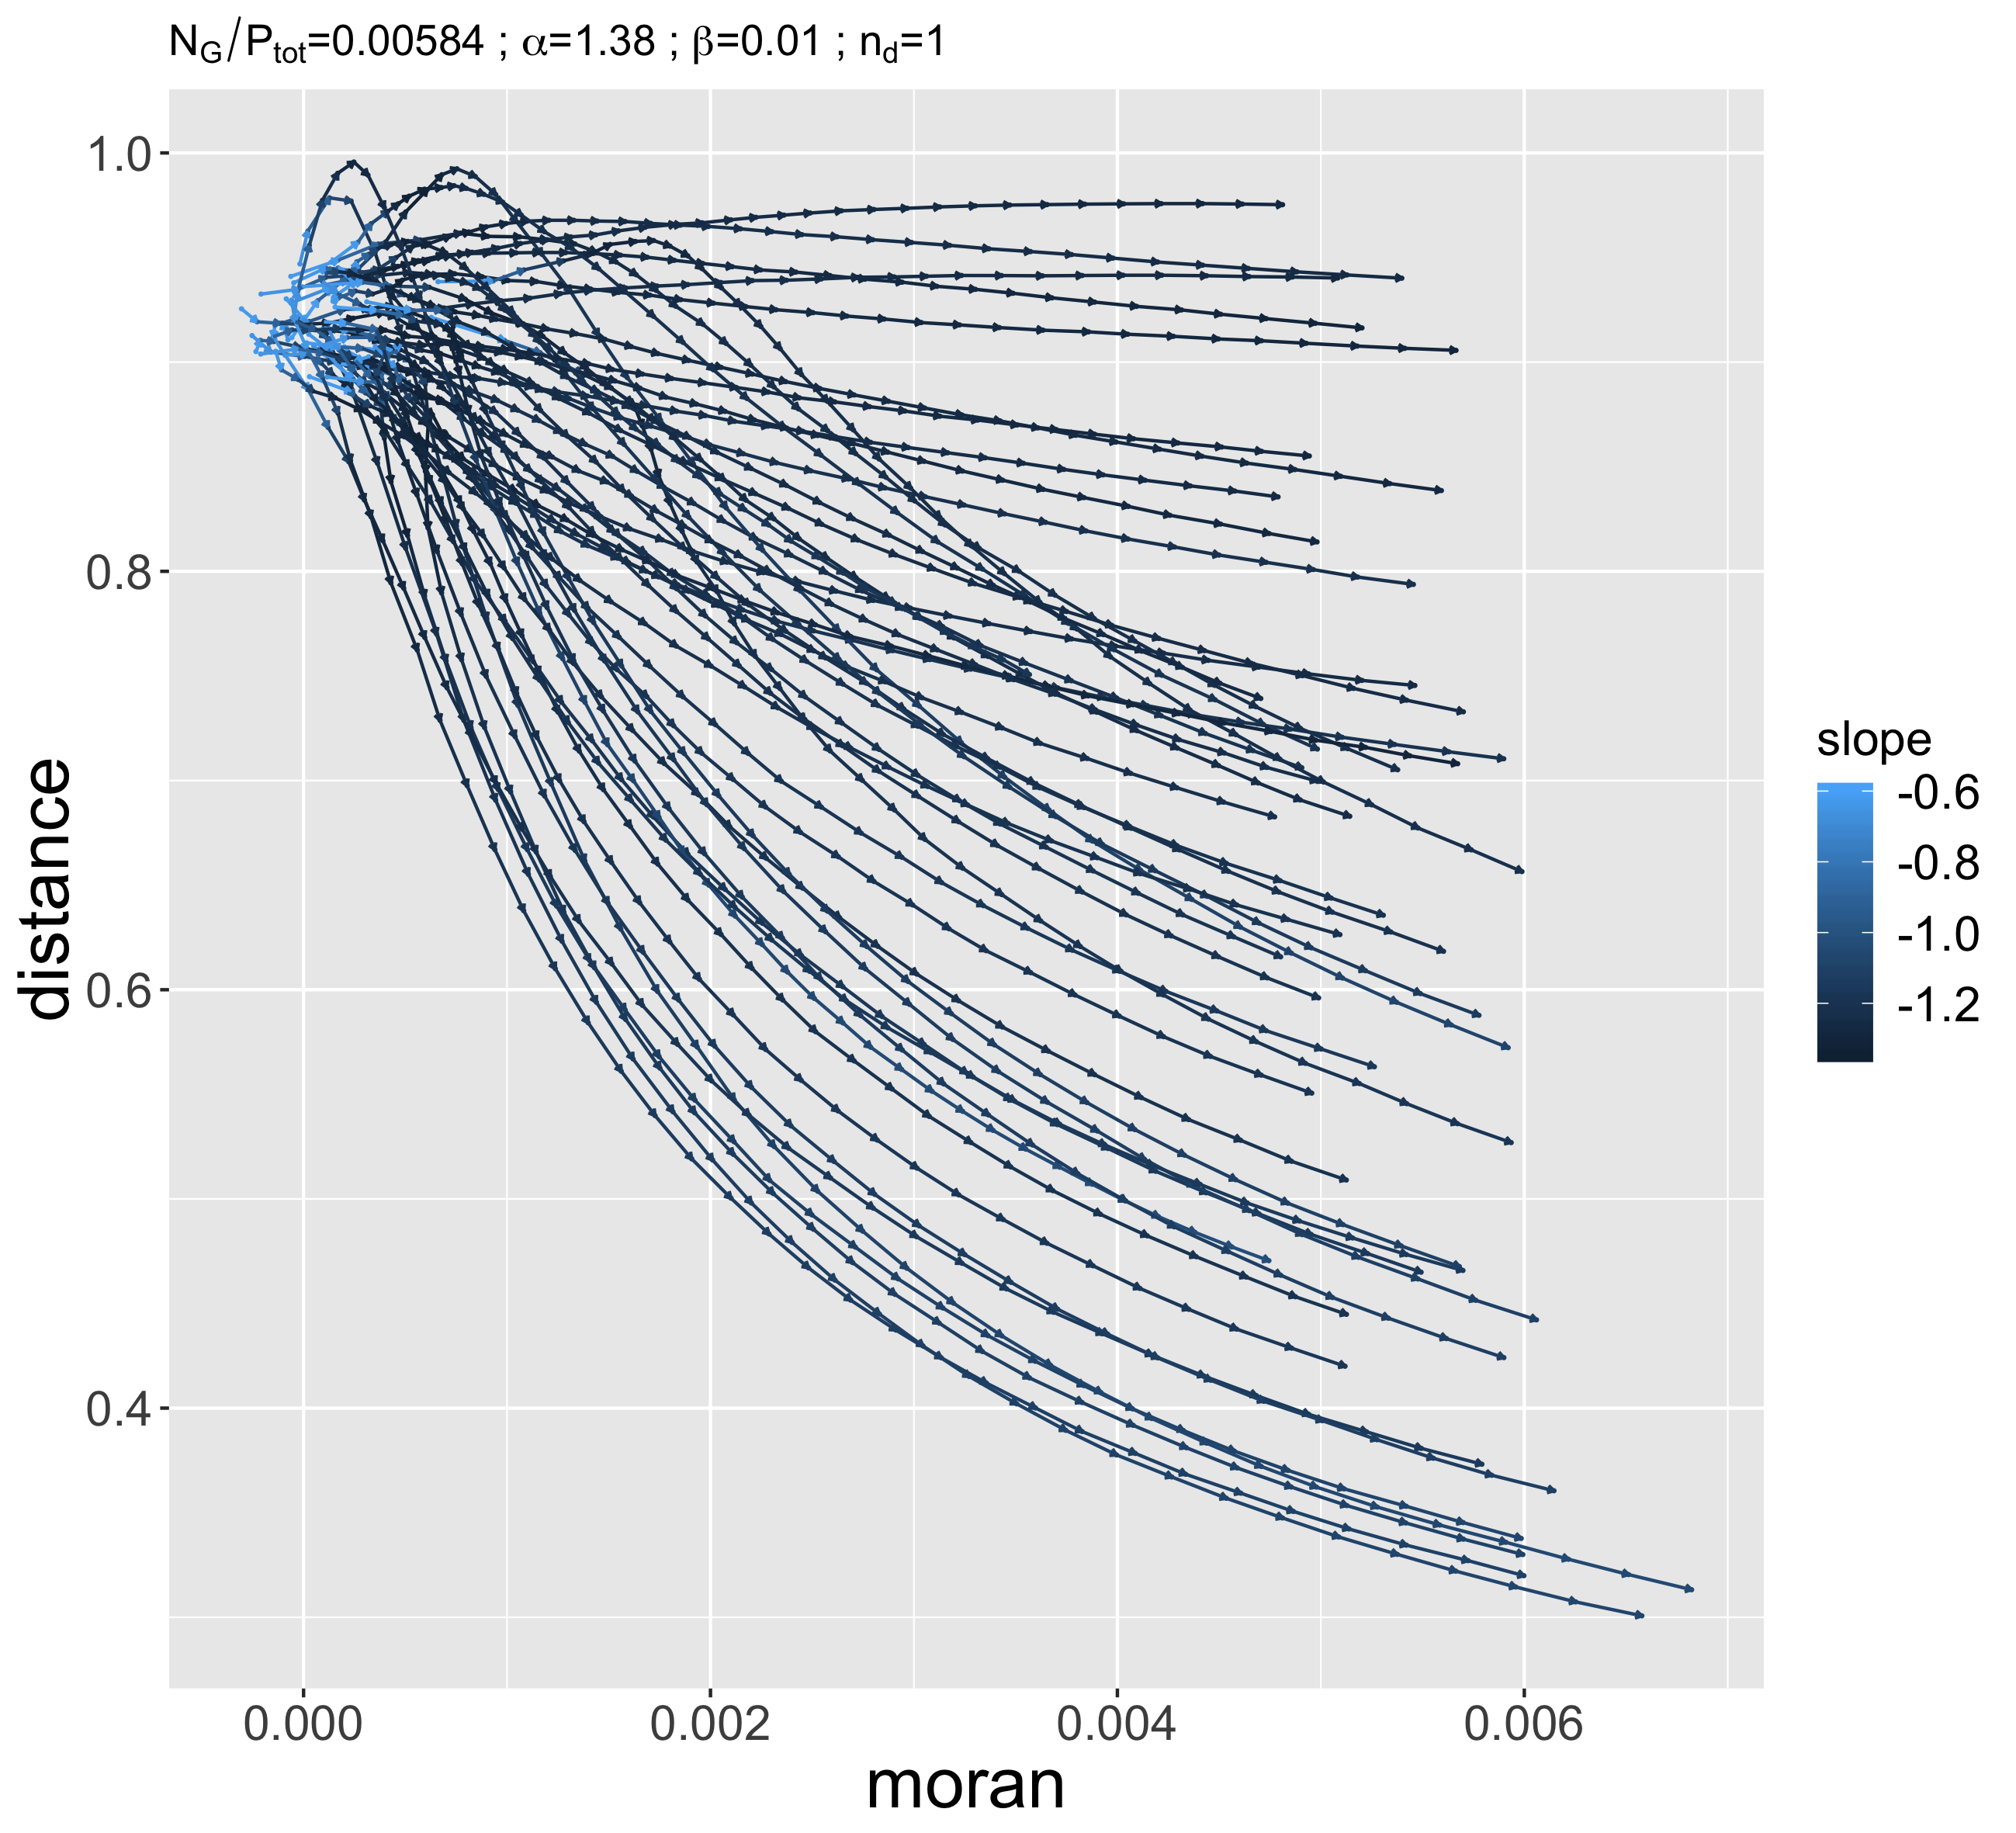
\includegraphics[width=0.7\linewidth]{figures/trajs_moran-dist_seed8578.png}
	\caption{\textbf{Temporal trajectories of the morphological indicators.} We show for a parameter point a sample of 50 trajectories in the morphological space (moran,distance), the color giving the level of hierarchy. In this configuration, the final variance is very large and trajectories sometimes cross others, confirming the path-dependence for morphological indicators.}
	\label{fig:morphotraj}
\end{figure}
%%%%%%%%%%%%%


% quand peut-on dire non ergod ?



%%%%%%%%%%%%%%%%%
\section{Complexité et co-évolution}
%%%%%%%%%%%%%%%%%


%\subsection{Co-évolution dans les systèmes territoriaux}

Une certaine approche des systèmes complexes territoriaux privilégie le concept de co-évolution. L'intrication forte des éléments présents au sein de ce qui peut être compris comme niches territoriales, au sens des niches écologiques de \cite{holland2012signals}, est une expression d'une co-évolution et donc d'une complexité au sein de ces niches. \cite{raimbault2018modeling} montre l'émergence de ces niches spatiales au sein d'un modèle de co-évolution entre villes et réseaux de transport à l'échelle macroscopique.

%\subsection{Non-stationnarité spatiale et co-évolution}

Nous explorons alors ici par des expériences de simulation le lien entre non-stationnarité spatiale, qui est également un marqueur de complexité spatiale, et émergence de niches au sein d'un modèle de morphogenèse hybride couplant développement urbain et réseau, introduit par~\cite{raimbault2014hybrid}.

Le modèle RBD~\citep{raimbault2014hybrid} couple de manière simple croissance urbaine et évolution du réseau viaire. La flexibilité des régimes qu'il permet de capturer fournit dans~\cite{raimbault2017identification} un test pour une méthode d'identification de causalités spatio-temporelles. Nous étendons ici cette méthode par une détection endogène des zones spatiales sur lesquelles sont estimées les corrélations, afin de montrer l'émergence de niches par la non-stationnarité. Pour une description précise du modèle ainsi que son utilisation comme producteur de données synthétiques, se référer à \cite{raimbault2018caracterisation}. Dans notre cas, les paramètres variables sont le nombre de centres initiaux $N_C$ ainsi que les poids relatifs des différentes variables explicatives $(w_c,w_r,w_d)$ (distance au centre, distance au réseau, densité) régissant la valeur locale lors de l'étalement urbain.

% Experimental setup:
%  - fixed distrib of field centers weight values ; repetitions with varying positions.
%  -> indicators : optimal number of niches ? "modularity" of these ? [idea : construct neighborhood network, weight = correlation, then modularity detection ?)

La non-stationnarité est introduite en faisant ces derniers paramètres de poids dans l'espace. Nous distinguons deux implémentations, étant donné des valeurs attribuées à chaque centre : (i) la valeur locale des poids est donnée par celle du centre le plus proche ; (ii) la valeur locale est la moyenne des valeurs des centres pondérée par les distances à ceux-ci.

Les niches spatiales sont détectées par classification non-supervisée sur les profils de corrélation retardées estimées localement dans l'espace, c'est-à-dire $(\rho_{\tau}\left[X_i,X_j\right])_{\tau,i,j}$ où $- \tau_M \leq \tau \leq  \tau_M$ avec $\tau_M = 5$. Les séries temporelles sont tronquées au dessous de $t_0 = 5$ et à un point spatial donné, les corrélations sont estimées sur les cellules dans un rayon de $r_0 = 10$, avec un pas spatial de $\delta x = 5$. Un algorithme des k-means est utilisé pour classifier les profils, avec un nombre de clusters $k = N_C$. Pour supprimer la stochasticité de la classification, celle-ci est répétée $b = 1000$ fois, et les mesures de performance sont estimées sur l'ensemble de ces réalisations de la classification.

%Distance entre partitions \cite{porumbel2011efficient} \cite{day1981complexity} \cite{gusfield2002partition} \cite{rossi2011partition}
Afin de quantifier la classification, une solution pourrait être d'étudier une distance à la partition définie par les zones de stationnarité. Cependant, la détermination d'une distance entre partitions est un problème NP-difficile \citep{day1981complexity} dont même les solutions optimales \citep{porumbel2011efficient} dépassent les capacités de calcul vu le nombre de réalisations. Nous utilisons donc les indicateurs suivants, capturant des propriétés attendues de niches spatiales : (i) distance cumulée entre les centroïdes de la classification et les centres, corrigée par la distance entre les centroïdes et celle entre les centres % formule ?
 ; (ii) rayon normalisé moyen des clusters ; (iii) distance moyenne entre les vecteurs de features utilisés pour la classification ; (iv) variance intra-cluster moyenne. Chaque indicateur est calculé sur la classification obtenue ainsi que sur un modèle nul donné par une redistribution aléatoire des étiquettes de cluster entre les points.
 
 
%%%%%%%%%%%%%%
\begin{figure}
	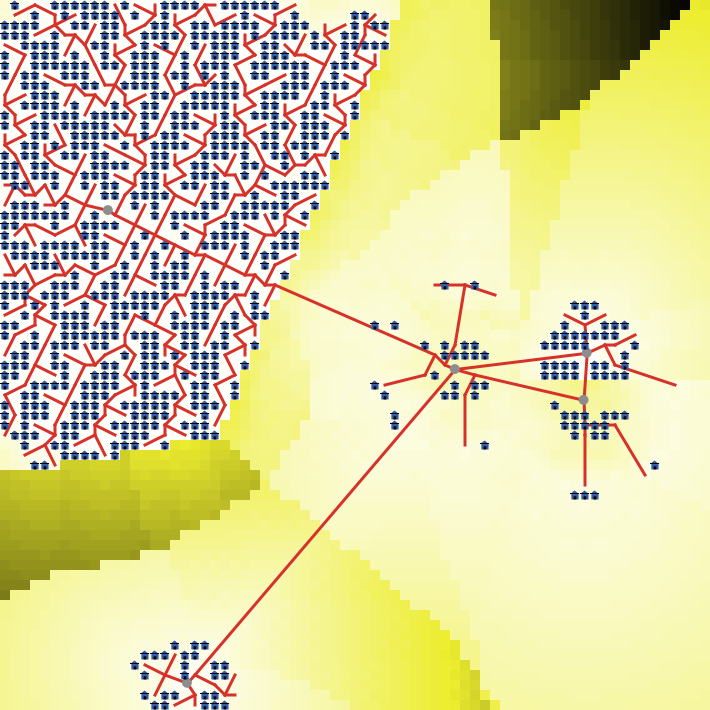
\includegraphics[width=0.49\textwidth]{figures/ex_0_tf30.png}
	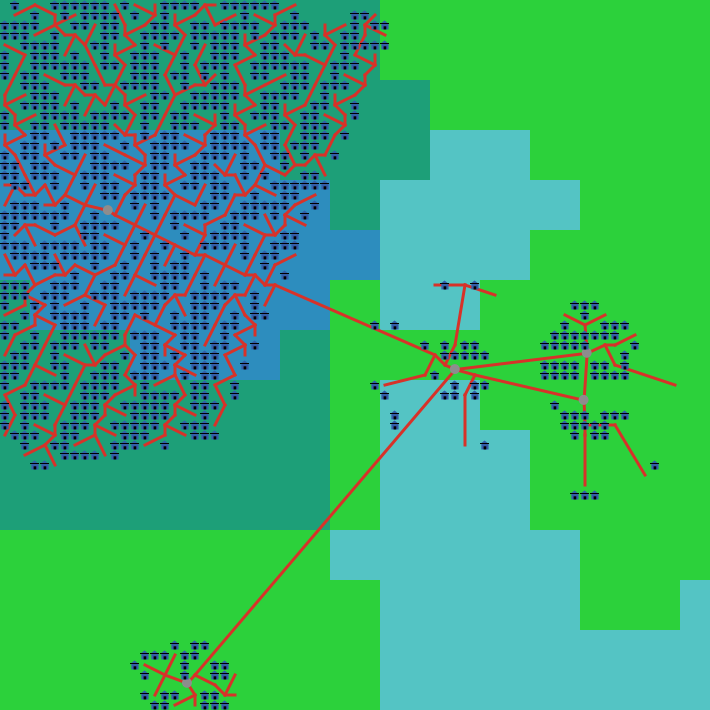
\includegraphics[width=0.49\textwidth]{figures/ex_0_tf30_rsclustering321.png}\\\bigskip
	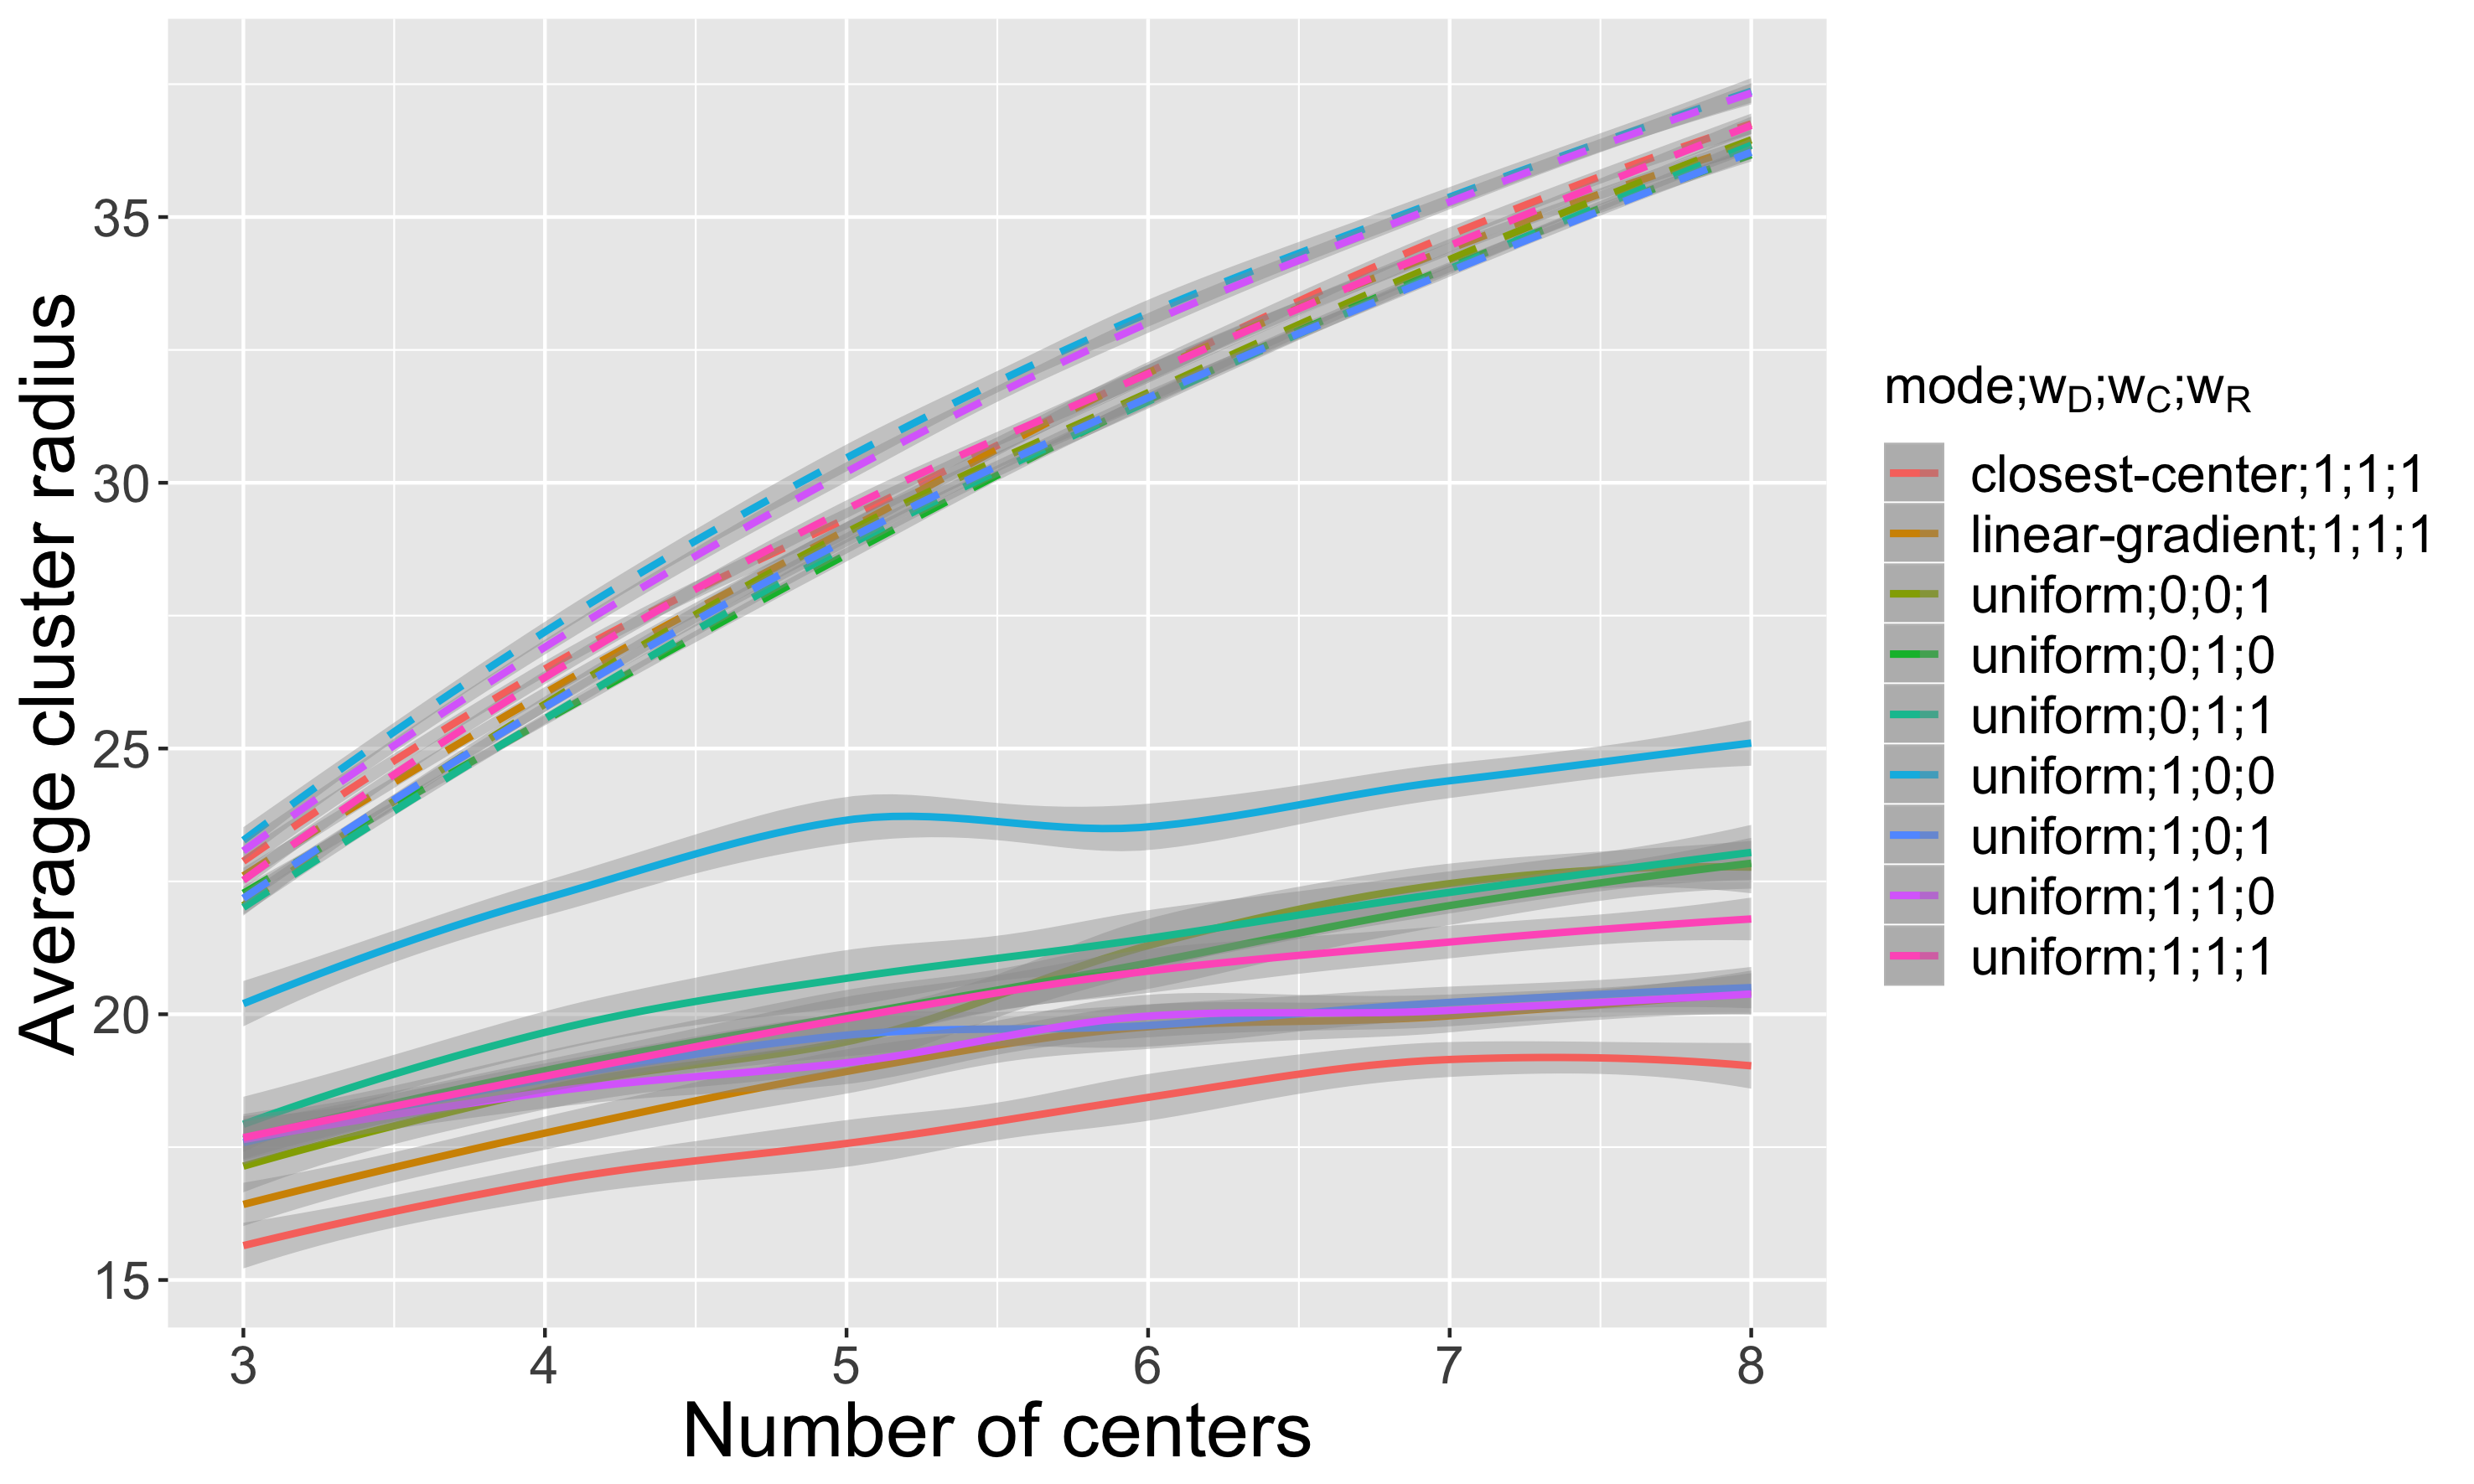
\includegraphics[width=0.49\textwidth]{figures/radius.png}
	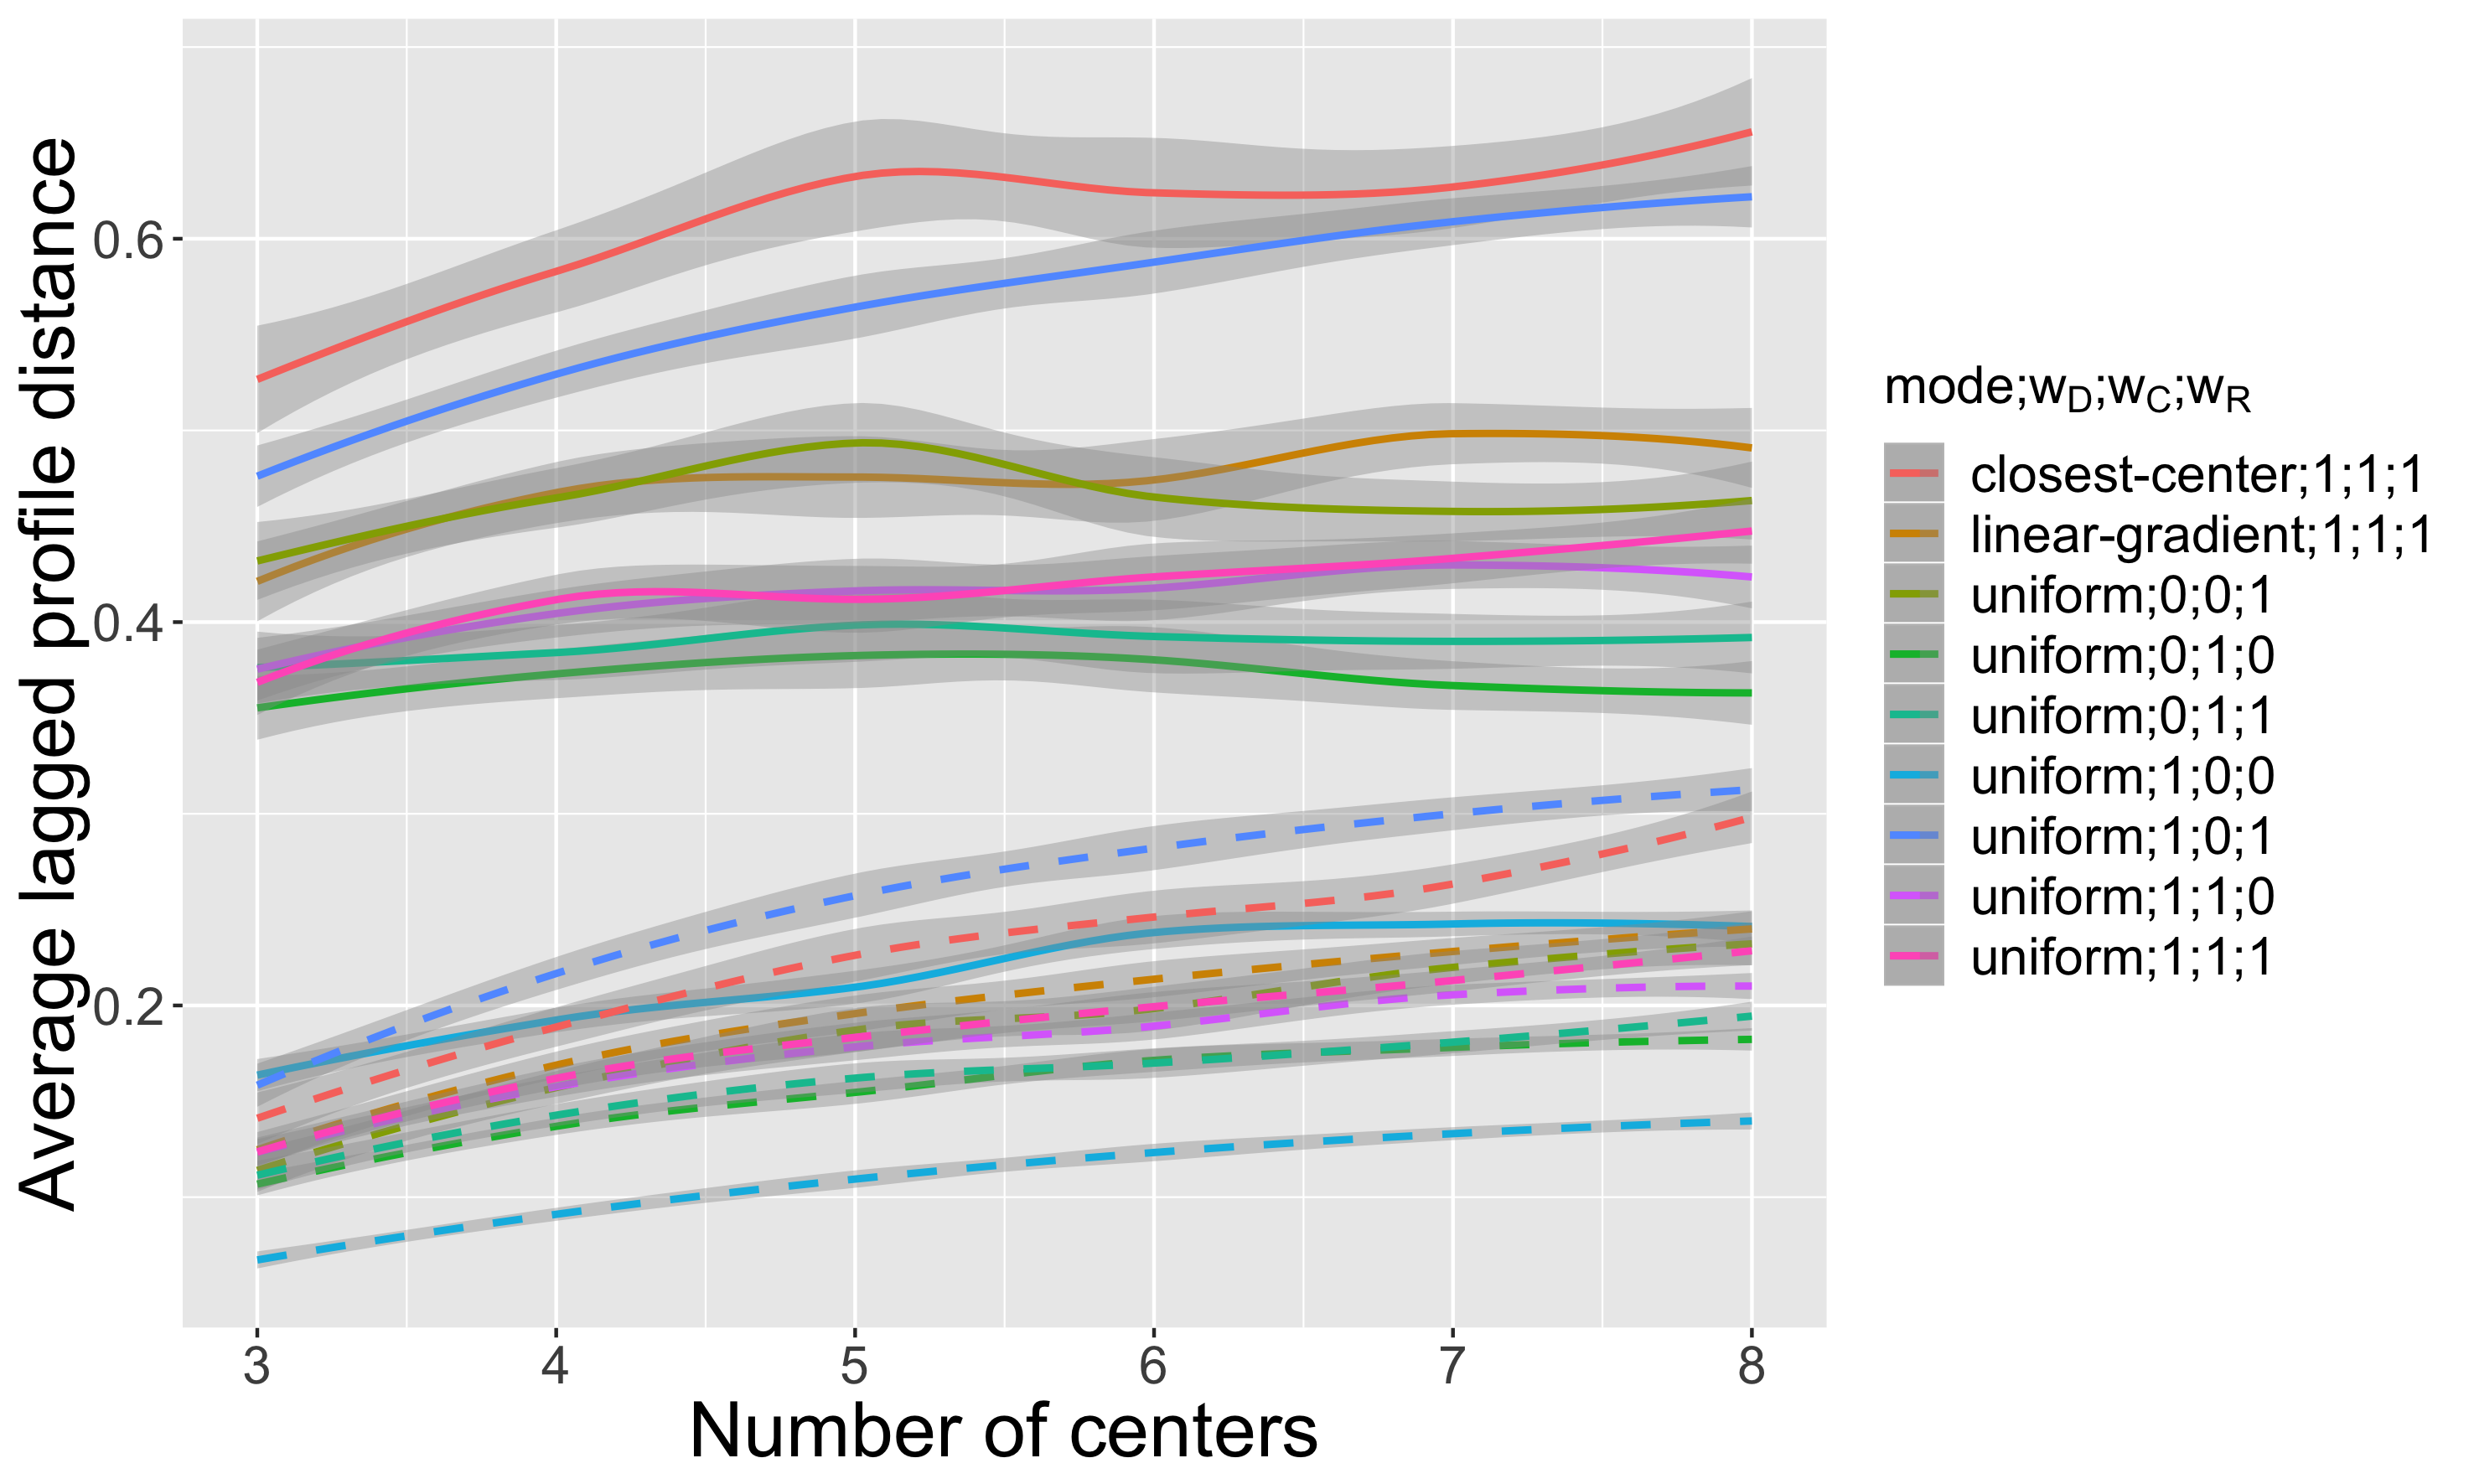
\includegraphics[width=0.49\textwidth]{figures/profiledisteucl.png}\\
	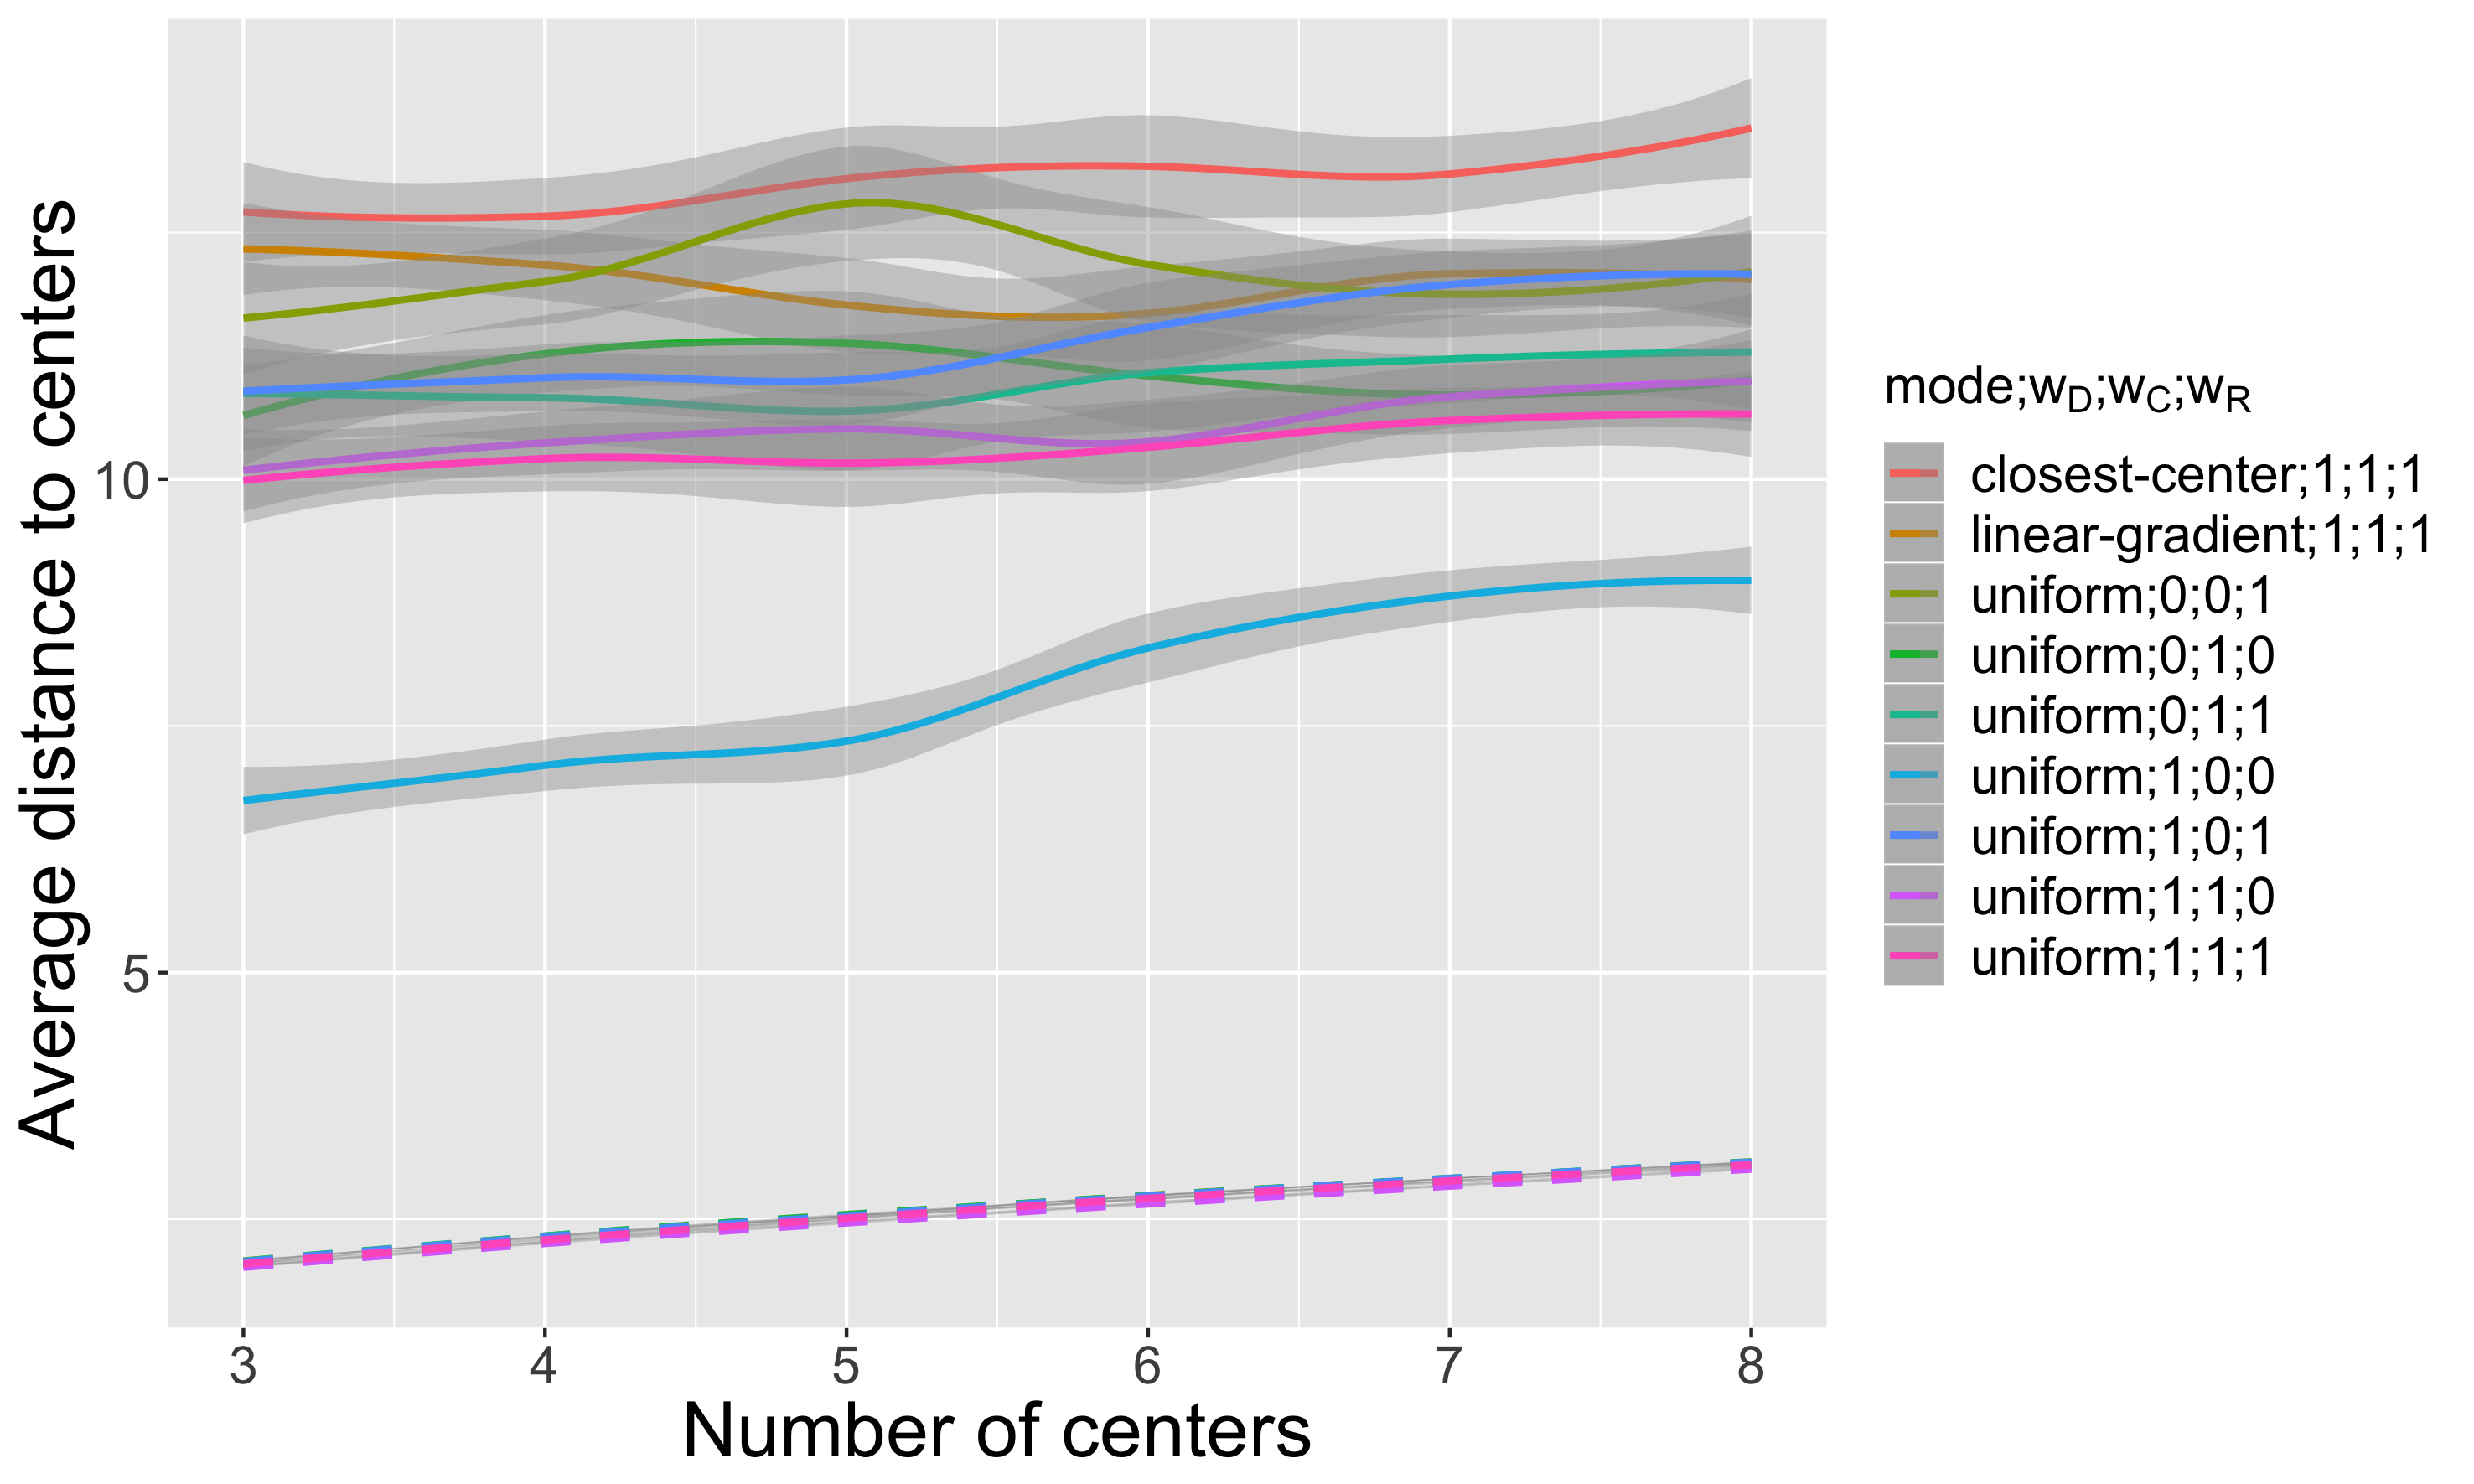
\includegraphics[width=0.49\textwidth]{figures/distance.png}
	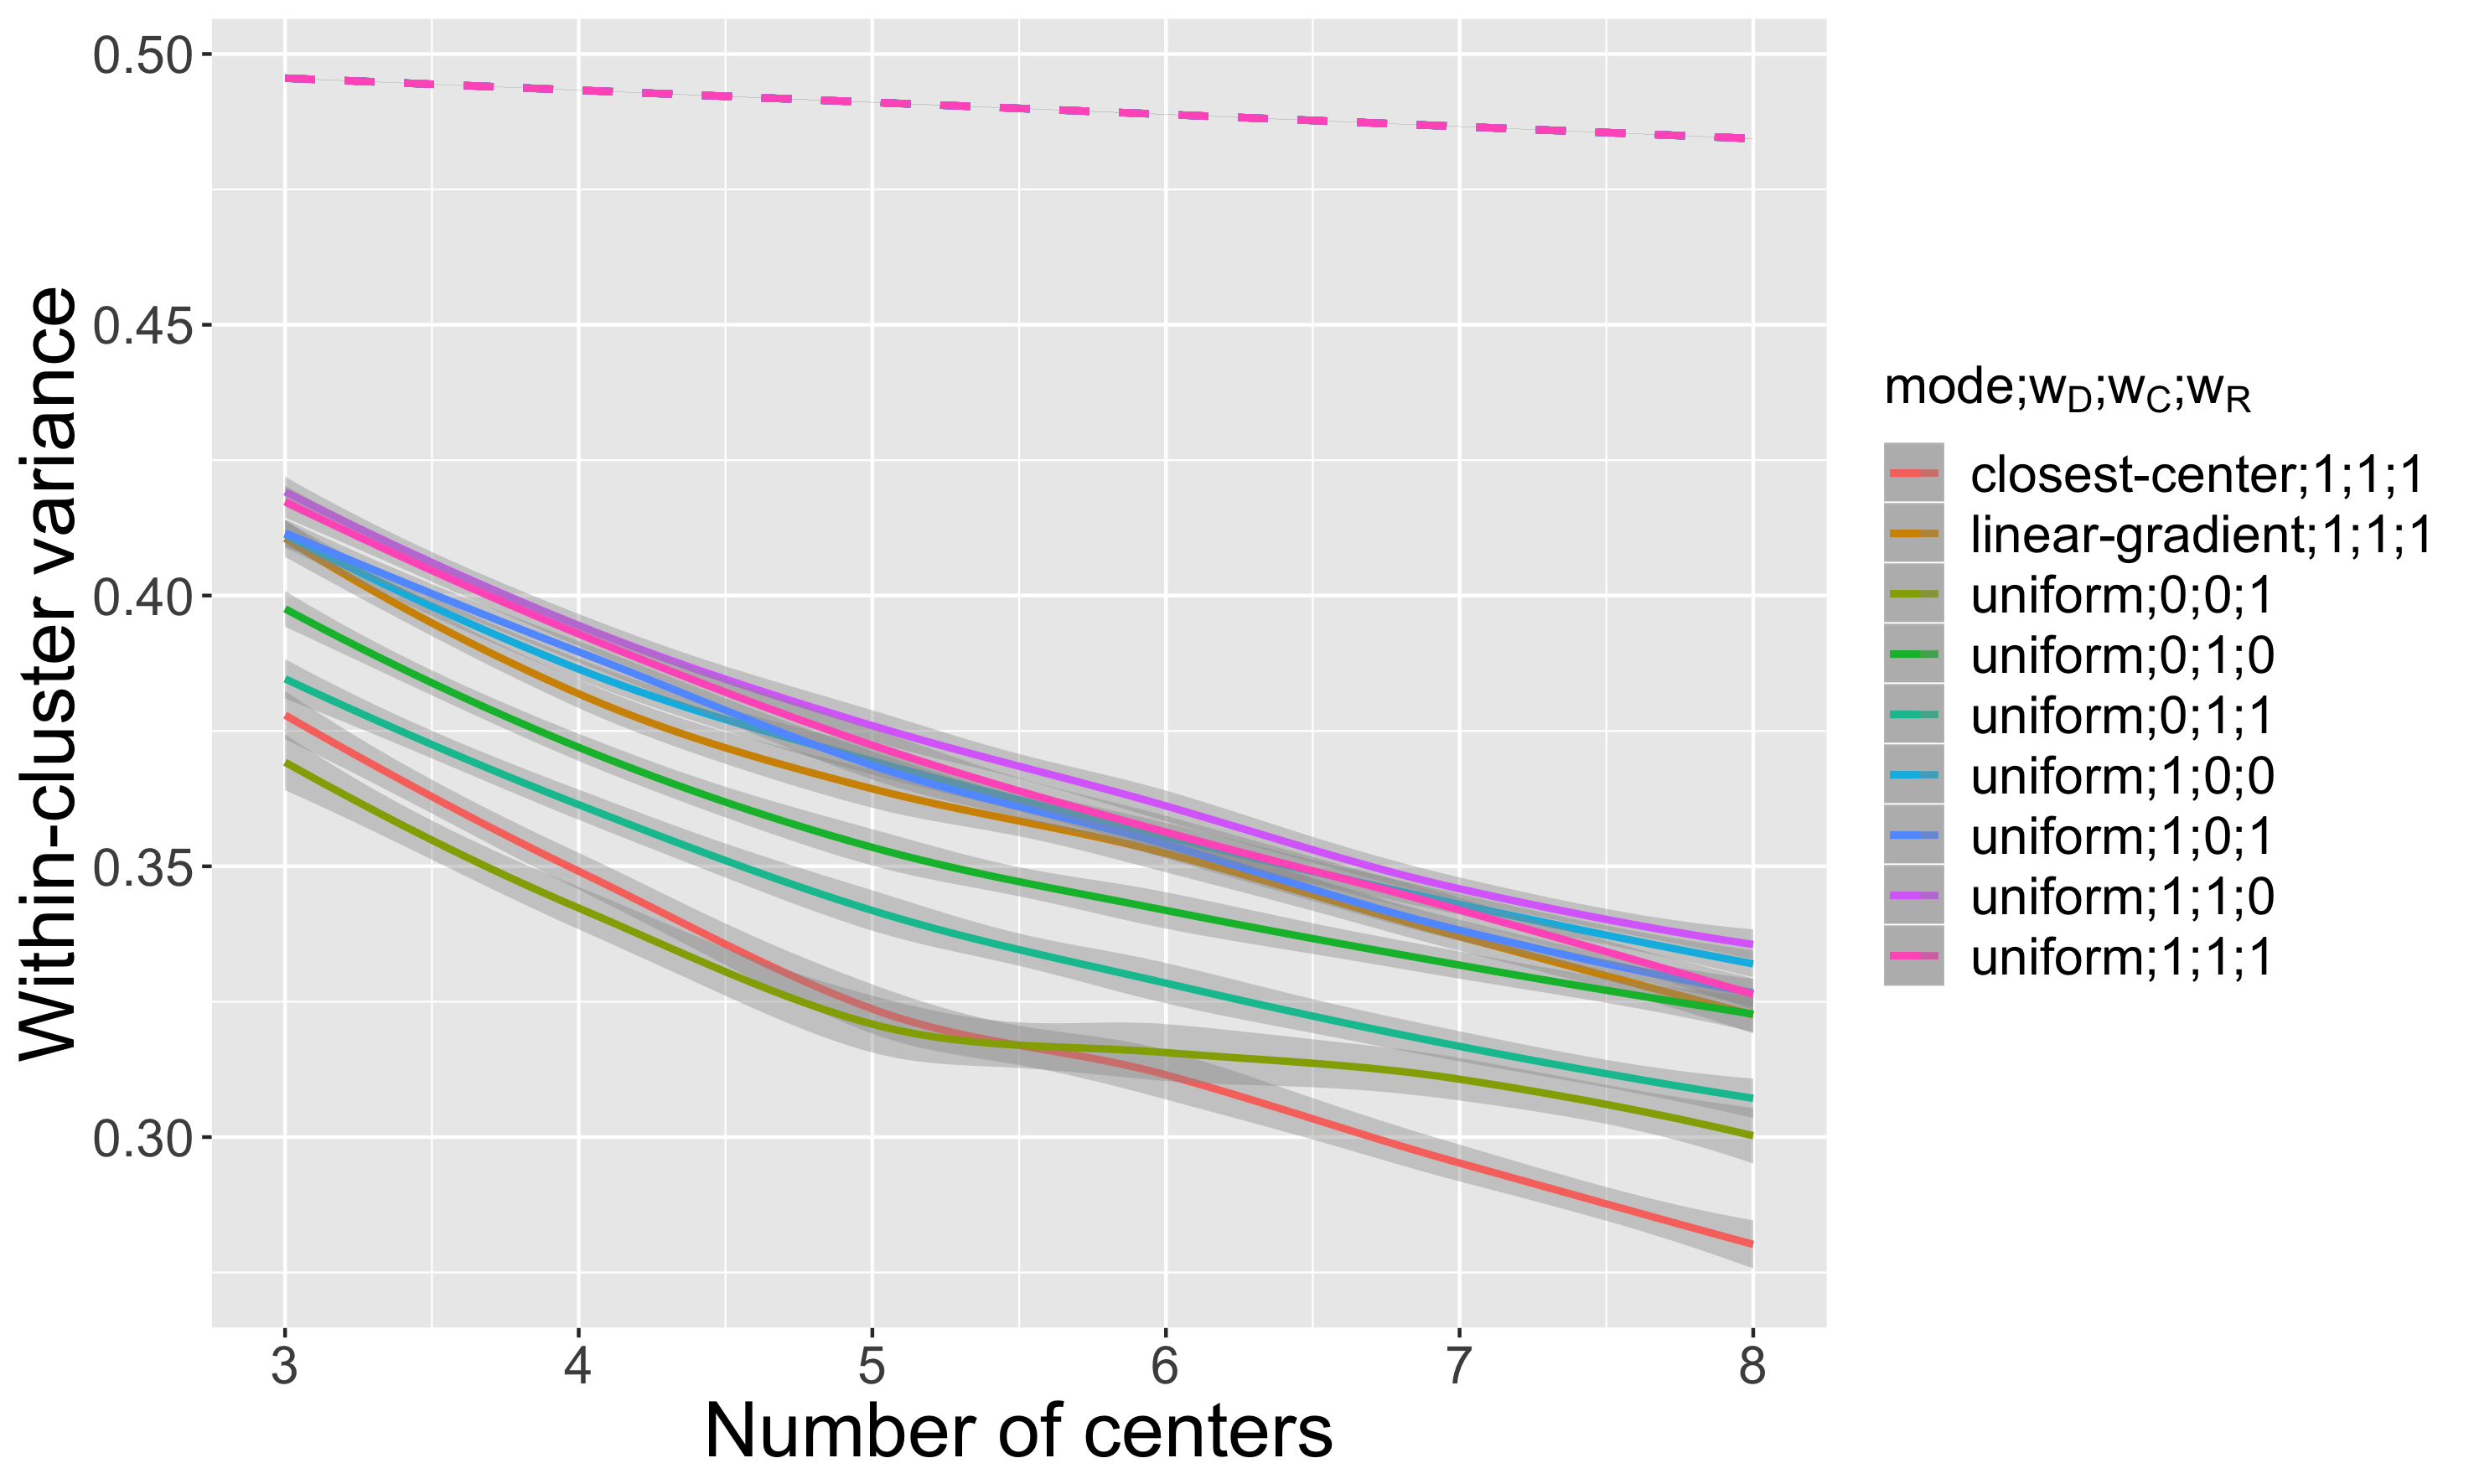
\includegraphics[width=0.49\textwidth]{figures/withinss.png}
	\caption{\textbf{Niches spatiales de co-évolution dans le modèle RBD.}\textit{(Haut gauche)} Configuration générée avec $N_C = 5$ centres et des paramètres non-stationnaires par centre le plus proche, tels que, dans un ordre de coordonnée verticale décroissante, les poids pour chaque centre sont $(w_d,w_r,w_c) = (0,1,0) ; (0,0,1) ; (1,0,1) ; (1,0,1) ; (0,0,1)$ ; \textit{(Haut droite)} Exemple de réalisation correspondante pour la classification par k-means, la couleur de cellule donnant le cluster. ; \textit{(Milieu gauche)} Rayon normalisé moyen des clusters, pour chaque mode et configuration de paramètres (couleur), ainsi que pour le modèle nul de cluster aléatoire (lignes pointillées) ; \textit{(Milieu droit)} Distance moyenne entre les profils de corrélations retardées pour les centroïdes des clusters ; \textit{(Bas gauche)} Distance moyenne des centroïdes aux centres ; \textit{(Bas droite)} Variance intra-cluster.}
	\label{fig:rbd}
\end{figure}
%%%%%%%%%%%%%%

 
 
Notre plan d'expérience compare les deux modalités de non-stationnarité (distributions aléatoires des poids) à la version uniforme du modèle prise pour l'ensemble des valeurs extrêmes des poids, le nombre de centres $N_C$ variant entre 3 et 8, et 100 réplications sont effectuées pour chaque point de paramètre. Nous montrons en Fig.~\ref{fig:rbd} un exemple de configuration obtenue dans le cas d'une non-stationnarité par centre le plus proche et la classification spatiale correspondante. La continuité spatiale des clusters est essentielle puisque ceux-ci correspondent alors aux niches de co-évolution. Les valeurs des indicateurs confirment l'existence systématique de ces niches. En effet, le rayon moyen, qui donne l'étalement spatial des clusters, est d'une part considérablement différent du modèle nul pour l'ensemble des paramètres, mais surtout significativement (au sens statistique) plus bas pour la non-stationnarité par centre plus proche par rapport à l'ensemble des configurations de contrôle. La non-stationnarité linéaire n'est quant à elle pas conclusive. Les autres indicateurs confirment l'émergence des niches: la distance entre profils des centroïdes est la plus grande dans le cas non-stationnaire par centre le plus proche, ce qui veut dire qu'il s'agit du cas où les clusters ont le plus de sens en termes de différentiations des caractéristiques. Cela correspond aussi à la plus basse variance intra-cluster, observée pour les plus grand nombres de centres. La distance moyenne des centroïdes aux centres est cependant la plus grande pour cette configuration, montrant que les niches ne coincident pas avec les zones de non-stationnarité, ce qui confirme que celles-ci sont bien émergentes et non juste la reproduction de la configuration initiale. Ainsi, cette expérience montre que la non-stationnarité spatiale mène à l'émergence de niches spatiales (qui ont une cohérence spatiale intrinsèque) pour les profils de corrélations retardées, et donc de niches de co-évolution au sens de \cite{raimbault2018caracterisation}. L'espace est encore une fois essentiel pour la production d'une complexité, cette fois au sens d'une co-évolution.







%\subsection{Detection des niches territoriales}

% for future paper ?

%Il est important dans ce cas de noter des approches complémentaires pour la détection de niches spatiales, qui peuvent faire l'object de développements futurs

% version GA
% -> for alife paper ?
%Soit $\mathbf{X}=\vec{x}_{1\leq i\leq N}$ les points générateurs des zones d'estimation (construites par triangulation de Dirichlet). Nous résolvons le problème d'optimisation
%\[
%\min_{N,\mathbf{X}} f(\tilde{\rho}_i)
%\]
%où la fonction $f$ donne un objectif en termes d'estimation de la corrélation (par exemple corrélation absolue moyenne $ - 1/N \sum_i \left| \rho_i \right|$, corrélation maximale $ - \max \left| \rho_i \right|$, niveau d'estimation en termes de taille des intervalles de confiance).

%En pratique, le problème est résolu de manière heuristique par algorithme génétique, à nombre fixé de centres variant dans $3\leq N \leq 10$ (sachant que le champ non-stationnaire est généré par un nombre fixe de centres $N=6$).


% version corr network
% -> not done either - does not work well

%Les niches territoriales sont détectées de la façon suivante: 
%\begin{enumerate}
%	\item Un réseau support est créé, avec des noeuds sur une grille de taille fixée ($k = 5$) et une connexion aux 8 plus proches voisins.
%	\item Une distance entre chaque couple de noeud voisin est calculée par
%	\[
%	d_{ij} = \sqrt{\sum_k (\tau_M^{(k)}(i) - \tau_M^{(k)}(j))^2}
%	\]
%	\item Le poids des liens du réseau est donné par $w_{ij} = \frac{1}{1 + d_{ij}^p}$
%	\item Une détection de communautés (algorithme de Louvain) est effectuée dans le réseau pondéré correspondant
%	\item La distance entre la partition obtenue et la partition correspondant à la non-stationnarité est calculée par diversité moyenne des profils de communautés en termes d'appartenance aux communautés de la partition opposée.
%\end{enumerate}
%


\section{Discussion}



Diverses approches de la complexité que nous n'avons pu aborder peuvent être suggérées en perspective, comme étant également typique des systèmes territoriaux et pouvant être liées à l'espace. Il pourrait par exemple exister un lien entre complexité computationnelle et caractère de grande déviation des configurations territoriales (impossibilité empirique en probabilité de les obtenir en force brute) : dans quelle mesure un système territorial est-il facile à générer par computation, et quelles propriétés peuvent expliquer cette possibilité ? En effet, à l'image des propriétés computationnelles de systèmes biologiques spatiaux auto-organisés comme le \emph{slime mould} qui sont capables de résoudre des problèmes NP-complets \citep{zhu2013amoeba}, les systèmes territoriaux pourrait en ce sens avoir une certaine intelligence, la question restant ouverte dans quelle mesure ceci est lié à sa configuration spatiale. Il pourrait aussi être suggéré un lien entre complexité informationnelle et diffusion de l'innovation dans les systèmes territoriaux \citep{favaro2011gibrat}. La diffusion de l'innovation est suggérée comme un moteur fondamental des dynamiques urbaines par la théorie évolutive urbaine. L'innovation est liée aux processus d'évolution culturelle \citep{Mesoudi25072017} et donc à une complexité informationnelle au sens de motifs non triviaux de transmission et traitement de l'information. La distribution spatiale de ces processus, et dans quelle mesure celle-ci influence ses propriétés, est une piste de développement importante pour l'étude de la complexité spatiale des systèmes territoriaux.


Le travail développé ici s'est cantonné à des considérations théoriques et des exemples jouets. La construction systématique, autant au sens de construction des concepts par revue systématique, que de construction de théories et méthodes articulant de manière pertinentes ces différents liens entre complexité et espace, reste une perspective ouverte pour des recherches futures. Nous concluons ainsi, suivant \cite{raimbault2017complexity}, que les systèmes territoriaux sont nécessairement au croisement de multiples complexités, et ajoutons, d'après les divers exemples développés ici, que leur caractère spatial prend une place importante dans l'émergence de celles-ci.
% TODO : rq : complexite aplique a la complexitee elle meme : meta et reflexivite
% rq : une autre facon de dire que la reflexivite est necessaire ?

% TODO cit perspectvisme applique et cybergeonetworks ?




%%%%%%%%%%%%%%%
\section*{Remerciements}

Les résultats obtenus dans cet article ont été calculés sur l'organisation virtuelle \texttt{vo.complex-system.eu} de l'European Grid Infrastructure (\texttt{http://www.egi.eu}). Nous remercions l'\textit{European Grid Infrastructure} et ses \textit{National Grid Initiatives} (France-Grilles en particulier) pour fournir le support technique et l'infrastructure.





%%%%%%%%%%%%%%%%%%%%
%% Biblio
%%%%%%%%%%%%%%%%%%%%
%\tiny

%\begin{multicols}{2}

%\setstretch{0.3}
%\setlength{\parskip}{-0.4em}


\bibliographystyle{apalike}
\bibliography{biblio}
%\end{multicols}



\end{document}
